% ****************************************************************************************
% ************************            ALGEBRA LINEAL          ****************************
% ****************************************************************************************

% =======================================================
% =======         HEADER FOR DOCUMENT        ============
% =======================================================
    % *********   DOCUMENT ITSELF   **************
    \documentclass[12pt, fleqn]{report}                             %Type of docuemtn and size of font and left eq
    \usepackage[margin=1.2in]{geometry}                             %Margins and Geometry pacakge
    \usepackage{ifthen}                                             %Allow simple programming
    \usepackage{hyperref}                                           %Create MetaData for a PDF and LINKS!
    \usepackage{pdfpages}                                           %Create MetaData for a PDF and LINKS!
    \hypersetup{pageanchor=false}                                   %Solve 'double page 1' warnings in build
    \setlength{\parindent}{0pt}                                     %Eliminate ugly indentation
    \author{Oscar Andrés Rosas}                                     %Who I am

    % *********   LANGUAJE AND UFT-8   *********
    \usepackage[spanish]{babel}                                     %Please use spanish
    \usepackage[utf8]{inputenc}                                     %Please use spanish - UFT
    \usepackage[T1]{fontenc}                                        %Please use spanish
    \usepackage{textcmds}                                           %Allow us to use quoutes
    \usepackage{changepage}                                         %Allow us to use identate paragraphs
    \usepackage{anyfontsize}                                        %All the sizes

    % *********   MATH AND HIS STYLE  *********
    \usepackage{ntheorem, amsmath, amssymb, amsfonts}               %All fucking math, I want all!
    \usepackage{mathrsfs, mathtools, empheq}                        %All fucking math, I want all!
    \usepackage{cancel}                                             %Negate symbol
    \usepackage{centernot}                                          %Allow me to negate a symbol
    \decimalpoint                                                   %Use decimal point

    % *********   GRAPHICS AND IMAGES *********
    \usepackage{graphicx}                                           %Allow to create graphics
    \usepackage{float}                                              %For images
    \usepackage{wrapfig}                                            %Allow to create images
    \graphicspath{ {Graphics/} }                                    %Where are the images :D

    % *********   LISTS AND TABLES ***********
    \usepackage{listings, listingsutf8}                             %We will be using code here
    \usepackage[inline]{enumitem}                                   %We will need to enumarate
    \usepackage{tasks}                                              %Horizontal lists
    \usepackage{longtable}                                          %Lets make tables awesome
    \usepackage{booktabs}                                           %Lets make tables awesome
    \usepackage{tabularx}                                           %Lets make tables awesome
    \usepackage{multirow}                                           %Lets make tables awesome
    \usepackage{multicol}                                           %Create multicolumns

    % *********   HEADERS AND FOOTERS ********
    \def\ProjectAuthorLink{https://github.com/SoyOscarRH}           %Just to keep it in line
    \def\ProjectNameLink{https://github.com/CompilandoConocimiento} %Just to keep it in line

    % *********   HEADERS AND FOOTERS ********
    \usepackage{fancyhdr}                                           %Lets make awesome headers/footers
    \pagestyle{fancy}                                               %Lets make awesome headers/footers
    \setlength{\headheight}{16pt}                                   %Top line
    \setlength{\parskip}{0.5em}                                     %Top line
    \renewcommand{\footrulewidth}{0.5pt}                            %Bottom line

    \lhead {                                                        %Left Header
        \hyperlink{chapter.\arabic{chapter}}                        %Make a link to the current chapter
        {\normalsize{\textsc{\nouppercase{\leftmark}}}}             %And fot it put the name
    }

    \rhead {                                                        %Right Header
        \hyperlink{section.\arabic{chapter}.\arabic{section}}       %Make a link to the current chapter
            {\footnotesize{\textsc{\nouppercase{\rightmark}}}}      %And fot it put the name
    }

    \rfoot{\textsc{\small{\hyperref[sec:Index]{Ve al Índice}}}}     %This will always be a footer  

    \fancyfoot[L]{                                                  %Algoritm for a changing footer
        \ifthenelse{\isodd{\value{page}}}                           %IF ODD PAGE:
            {\href{https://compilandoconocimiento.com/nosotros/}    %DO THIS:
                {\footnotesize                                      %Send the page
                    {\textsc{Oscar Andrés Rosas}}}}                 %Send the page
            {\href{https://compilandoconocimiento.com}              %ELSE DO THIS: 
                {\footnotesize                                      %Send the author
                    {\textsc{Compilando Conocimiento}}}}            %Send the author
    }
    
    
    
% ========================================
% ===========   COMMANDS    ==============
% ========================================

    % =========================================
    % =======   NEW ENVIRONMENTS   ============
    % =========================================
    \newenvironment{Indentation}[1][0.75em]                         %Use: \begin{Inde...}[Num]...\end{Inde...}
        {\begin{adjustwidth}{#1}{}}                                 %If you dont put nothing i will use 0.75 em
        {\end{adjustwidth}}                                         %This indentate a paragraph
    \newenvironment{SmallIndentation}[1][0.75em]                    %Use: The same that we upper one, just 
        {\begin{adjustwidth}{#1}{}\begin{footnotesize}}             %footnotesize size of letter by default
        {\end{footnotesize}\end{adjustwidth}}                       %that's it

    \newenvironment{MultiLineEquation}[1]                           %Use: To create MultiLine equations
        {\begin{equation}\begin{alignedat}{#1}}                     %Use: \begin{Multi..}{Num. de Columnas}
        {\end{alignedat}\end{equation}}                             %And.. that's it!
    \newenvironment{MultiLineEquation*}[1]                          %Use: To create MultiLine equations
        {\begin{equation*}\begin{alignedat}{#1}}                    %Use: \begin{Multi..}{Num. de Columnas}
        {\end{alignedat}\end{equation*}}                            %And.. that's it!
    

    % =========================================
    % == GENERAL TEXT & SYMBOLS ENVIRONMENTS ==
    % =========================================
    
    % =====  TEXT  ======================
    \newcommand \Quote {\qq}                                        %Use: \Quote to use quotes
    \newcommand \Over {\overline}                                   %Use: \Bar to use just for short
    \newcommand \ForceNewLine {$\Space$\\}                          %Use it in theorems for example

    % =====  SPACES  ====================
    \DeclareMathOperator \Space {\quad}                             %Use: \Space for a cool mega space
    \DeclareMathOperator \MegaSpace {\quad \quad}                   %Use: \MegaSpace for a cool mega mega space
    \DeclareMathOperator \MiniSpace {\;}                            %Use: \Space for a cool mini space
    
    % =====  MATH TEXT  =================
    \newcommand \Such {\MiniSpace | \MiniSpace}                     %Use: \Such like in sets
    \newcommand \Also {\MiniSpace \text{y} \MiniSpace}              %Use: \Also so it's look cool
    \newcommand \Remember[1]{\Space\text{\scriptsize{#1}}}          %Use: \Remember so it's look cool
    
    % =====  THEOREMS  ==================
    \newtheorem{Theorem}{Teorema}[section]                          %Use: \begin{Theorem}[Name]\label{Nombre}...
    \newtheorem{Corollary}{Colorario}[Theorem]                      %Use: \begin{Corollary}[Name]\label{Nombre}...
    \newtheorem{Lemma}[Theorem]{Lemma}                              %Use: \begin{Lemma}[Name]\label{Nombre}...
    \newtheorem{Definition}{Definición}[section]                    %Use: \begin{Definition}[Name]\label{Nombre}...
    \theoremstyle{break}                                            %THEOREMS START 1 SPACE AFTER

    % =====  LOGIC  =====================
    \newcommand \lIff {\leftrightarrow}                             %Use: \lIff for logic iff
    \newcommand \lEqual {\MiniSpace \Leftrightarrow \MiniSpace}     %Use: \lEqual for a logic double arrow
    \newcommand \lInfire {\MiniSpace \Rightarrow \MiniSpace}        %Use: \lInfire for a logic infire
    \newcommand \lLongTo {\longrightarrow}                          %Use: \lLongTo for a long arrow

    % =====  FAMOUS SETS  ===============
    \DeclareMathOperator \Naturals     {\mathbb{N}}                 %Use: \Naturals por Notation
    \DeclareMathOperator \Primes       {\mathbb{P}}                 %Use: \Primes por Notation
    \DeclareMathOperator \Integers     {\mathbb{Z}}                 %Use: \Integers por Notation
    \DeclareMathOperator \Racionals    {\mathbb{Q}}                 %Use: \Racionals por Notation
    \DeclareMathOperator \Reals        {\mathbb{R}}                 %Use: \Reals por Notation
    \DeclareMathOperator \Complexs     {\mathbb{C}}                 %Use: \Complex por Notation
    \DeclareMathOperator \GenericField {\mathbb{F}}                 %Use: \GenericField por Notation
    \DeclareMathOperator \VectorSet    {\mathbb{V}}                 %Use: \VectorSet por Notation
    \DeclareMathOperator \SubVectorSet {\mathbb{W}}                 %Use: \SubVectorSet por Notation

    % =====  CONTAINERS   ===============
    \newcommand{\Set}[1]{\left\{ \; #1 \; \right\}}                 %Use: \Set {Info} for INTELLIGENT space 
    \newcommand{\bigSet}[1]{\big\{ \; #1 \; \big\}}                 %Use: \bigSet  {Info} for space 
    \newcommand{\BigSet}[1]{\Big\{ \; #1 \; \Big\}}                 %Use: \BigSet  {Info} for space 
    \newcommand{\biggSet}[1]{\bigg\{ \; #1 \; \bigg\}}              %Use: \biggSet {Info} for space 
    \newcommand{\BiggSet}[1]{\Bigg\{ \; #1 \; \Bigg\}}              %Use: \BiggSet {Info} for space 
    
    \newcommand{\Brackets}[1]{\left[ #1 \right]}                    %Use: \Brackets {Info} for INTELLIGENT space
    \newcommand{\bigBrackets}[1]{\big[ \; #1 \; \big]}              %Use: \bigBrackets  {Info} for space 
    \newcommand{\BigBrackets}[1]{\Big[ \; #1 \; \Big]}              %Use: \BigBrackets  {Info} for space 
    \newcommand{\biggBrackets}[1]{\bigg[ \; #1 \; \bigg]}           %Use: \biggBrackets {Info} for space 
    \newcommand{\BiggBrackets}[1]{\Bigg[ \; #1 \; \Bigg]}           %Use: \BiggBrackets {Info} for space 
    
    \newcommand{\Wrap}[1]{\left( #1 \right)}                        %Use: \Wrap {Info} for INTELLIGENT space
    \newcommand{\bigWrap}[1]{\big( \; #1 \; \big)}                  %Use: \bigBrackets  {Info} for space 
    \newcommand{\BigWrap}[1]{\Big( \; #1 \; \Big)}                  %Use: \BigBrackets  {Info} for space 
    \newcommand{\biggWrap}[1]{\bigg( \; #1 \; \bigg)}               %Use: \biggBrackets {Info} for space 
    \newcommand{\BiggWrap}[1]{\Bigg( \; #1 \; \Bigg)}               %Use: \BiggBrackets {Info} for space 

    % =====  BETTERS MATH COMMANDS   =====
    \newcommand{\pfrac}[2]{\Wrap{\dfrac{#1}{#2}}}                   %Use: Put fractions in parentesis

    % =========================================
    % ====   LINEAL ALGEBRA & VECTORS    ======
    % =========================================

    % ===== UNIT VECTORS  ================
    \newcommand{\hati} {\hat{\imath}}                               %Use: \hati for unit vector    
    \newcommand{\hatj} {\hat{\jmath}}                               %Use: \hatj for unit vector    
    \newcommand{\hatk} {\hat{k}}                                    %Use: \hatk for unit vector

    % ===== MAGNITUDE  ===================
    \newcommand{\abs}[1]{\left\lvert #1 \right\lvert}               %Use: \abs{expression} for |x|
    \newcommand{\Abs}[1]{\left\lVert #1 \right\lVert}               %Use: \Abs{expression} for ||x||
    \newcommand{\Mag}[1]{\left| #1 \right|}                         %Use: \Mag {Info} 
    
    \DeclareMathOperator \LinealTransformation {\mathcal{T}}        %Use: \LinealTransformation for a cool T
    \newcommand{\bVec}[1]{\mathbf{#1}}                              %Use for bold type of vector
    \newcommand{\lVec}[1]{\overrightarrow{#1}}                      %Use for a long arrow over a vector
    \newcommand{\uVec}[1]{\mathbf{\hat{#1}}}                        %Use: Unitary Vector Example: $\uVec{i}

    % ===== ALL FOR DOT PRODUCT  =========
    \makeatletter                                                   %WTF! IS THIS
    \newcommand*\dotP{\mathpalette\dotP@{.5}}                       %Use: \dotP for dot product
    \newcommand*\dotP@[2] {\mathbin {                               %WTF! IS THIS            
        \vcenter{\hbox{\scalebox{#2}{$\m@th#1\bullet$}}}}           %WTF! IS THIS
    }                                                               %WTF! IS THIS
    \makeatother                                                    %WTF! IS THIS

    % === WRAPPERS FOR COLUMN VECTOR ===
    \newcommand{\pVector}[1]                                        %Use: \pVector {Matrix Notation} use parentesis
        { \ensuremath{\begin{pmatrix}#1\end{pmatrix}} }             %Example: \pVector{a\\b\\c} or \pVector{a&b&c} 
    \newcommand{\lVector}[1]                                        %Use: \lVector {Matrix Notation} use a abs 
        { \ensuremath{\begin{vmatrix}#1\end{vmatrix}} }             %Example: \lVector{a\\b\\c} or \lVector{a&b&c} 
    \newcommand{\bVector}[1]                                        %Use: \bVector {Matrix Notation} use a brackets 
        { \ensuremath{\begin{bmatrix}#1\end{bmatrix}} }             %Example: \bVector{a\\b\\c} or \bVector{a&b&c} 
    \newcommand{\Vector}[1]                                         %Use: \Vector {Matrix Notation} no parentesis
        { \ensuremath{\begin{matrix}#1\end{matrix}} }               %Example: \Vector{a\\b\\c} or \Vector{a&b&c}

    % === MAKE MATRIX BETTER  =========
    \makeatletter                                                   %Example: \begin{matrix}[cc|c]
    \renewcommand*\env@matrix[1][*\c@MaxMatrixCols c] {             %WTF! IS THIS
        \hskip -\arraycolsep                                        %WTF! IS THIS
        \let\@ifnextchar\new@ifnextchar                             %WTF! IS THIS
        \array{#1}                                                  %WTF! IS THIS
    }                                                               %WTF! IS THIS
    \makeatother                                                    %WTF! IS THIS

    % =========================================
    % =======   FAMOUS FUNCTIONS   ============
    % =========================================

    % == TRIGONOMETRIC FUNCTIONS  ====
    \newcommand{\Cos}[1]{\cos\Wrap{#1}}                             %Simple wrappers
    \newcommand{\Sin}[1]{\sin\Wrap{#1}}                             %Simple wrappers
    \newcommand{\Tan}[1]{tan\Wrap{#1}}                              %Simple wrappers
    
    \newcommand{\Sec}[1]{sec\Wrap{#1}}                              %Simple wrappers
    \newcommand{\Csc}[1]{csc\Wrap{#1}}                              %Simple wrappers
    \newcommand{\Cot}[1]{cot\Wrap{#1}}                              %Simple wrappers

    % === COMPLEX ANALYSIS TRIG ======
    \newcommand \Cis[1]  {\Cos{#1} + i \Sin{#1}}                    %Use: \Cis for cos(x) + i sin(x)
    \newcommand \pCis[1] {\Wrap{\Cis{#1}}}                          %Use: \pCis for the same with parantesis
    \newcommand \bCis[1] {\Brackets{\Cis{#1}}}                      %Use: \bCis for the same with Brackets


    % =========================================
    % ===========     CALCULUS     ============
    % =========================================

    % ====== TRANSFORMS =============
    \newcommand{\FourierT}[1]{\mathscr{F} \left\{ #1 \right\} }     %Use: \FourierT {Funtion}
    \newcommand{\InvFourierT}[1]{\mathscr{F}^{-1}\left\{#1\right\}} %Use: \InvFourierT {Funtion}

    % ====== DERIVATIVES ============
    \newcommand \MiniDerivate[1][x] {\dfrac{d}{d #1}}               %Use: \MiniDerivate[var] for simple use [var]
    \newcommand \Derivate[2] {\dfrac{d \; #1}{d #2}}                %Use: \Derivate [f(x)][x]
    \newcommand \MiniUpperDerivate[2] {\dfrac{d^{#2}}{d#1^{#2}}}    %Mini Derivate High Orden Derivate -- [x][pow]
    \newcommand \UpperDerivate[3] {\dfrac{d^{#3} \; #1}{d#2^{#3}}}  %Complete High Orden Derivate -- [f(x)][x][pow]
    
    \newcommand \MiniPartial[1][x] {\dfrac{\partial}{\partial #1}}  %Use: \MiniDerivate for simple use [var]
    \newcommand \Partial[2] {\dfrac{\partial \; #1}{\partial #2}}   %Complete Partial Derivate -- [f(x)][x]
    \newcommand \MiniUpperPartial[2]                                %Mini Derivate High Orden Derivate -- [x][pow] 
        {\dfrac{\partial^{#2}}{\partial #1^{#2}}}                   %Mini Derivate High Orden Derivate
    \newcommand \UpperPartial[3]                                    %Complete High Orden Derivate -- [f(x)][x][pow]
        {\dfrac{\partial^{#3} \; #1}{\partial#2^{#3}}}              %Use: \UpperDerivate for simple use

    \DeclareMathOperator \Evaluate  {\Big|}                         %Use: \Evaluate por Notation

    % =========================================
    % ========    GENERAL STYLE     ===========
    % =========================================
    
    % =====  COLORS ==================
    \definecolor{RedMD}{HTML}{F44336}                               %Use: Color :D        
    \definecolor{Red100MD}{HTML}{FFCDD2}                            %Use: Color :D        
    \definecolor{Red200MD}{HTML}{EF9A9A}                            %Use: Color :D        
    \definecolor{Red300MD}{HTML}{E57373}                            %Use: Color :D        
    \definecolor{Red700MD}{HTML}{D32F2F}                            %Use: Color :D 

    \definecolor{PurpleMD}{HTML}{9C27B0}                            %Use: Color :D        
    \definecolor{Purple100MD}{HTML}{E1BEE7}                         %Use: Color :D        
    \definecolor{Purple200MD}{HTML}{EF9A9A}                         %Use: Color :D        
    \definecolor{Purple300MD}{HTML}{BA68C8}                         %Use: Color :D        
    \definecolor{Purple700MD}{HTML}{7B1FA2}                         %Use: Color :D 

    \definecolor{IndigoMD}{HTML}{3F51B5}                            %Use: Color :D        
    \definecolor{Indigo100MD}{HTML}{C5CAE9}                         %Use: Color :D        
    \definecolor{Indigo200MD}{HTML}{9FA8DA}                         %Use: Color :D        
    \definecolor{Indigo300MD}{HTML}{7986CB}                         %Use: Color :D        
    \definecolor{Indigo700MD}{HTML}{303F9F}                         %Use: Color :D 

    \definecolor{BlueMD}{HTML}{2196F3}                              %Use: Color :D        
    \definecolor{Blue100MD}{HTML}{BBDEFB}                           %Use: Color :D        
    \definecolor{Blue200MD}{HTML}{90CAF9}                           %Use: Color :D        
    \definecolor{Blue300MD}{HTML}{64B5F6}                           %Use: Color :D        
    \definecolor{Blue700MD}{HTML}{1976D2}                           %Use: Color :D        
    \definecolor{Blue900MD}{HTML}{0D47A1}                           %Use: Color :D  

    \definecolor{CyanMD}{HTML}{00BCD4}                              %Use: Color :D        
    \definecolor{Cyan100MD}{HTML}{B2EBF2}                           %Use: Color :D        
    \definecolor{Cyan200MD}{HTML}{80DEEA}                           %Use: Color :D        
    \definecolor{Cyan300MD}{HTML}{4DD0E1}                           %Use: Color :D        
    \definecolor{Cyan700MD}{HTML}{0097A7}                           %Use: Color :D        
    \definecolor{Cyan900MD}{HTML}{006064}                           %Use: Color :D 

    \definecolor{TealMD}{HTML}{009688}                              %Use: Color :D        
    \definecolor{Teal100MD}{HTML}{B2DFDB}                           %Use: Color :D        
    \definecolor{Teal200MD}{HTML}{80CBC4}                           %Use: Color :D        
    \definecolor{Teal300MD}{HTML}{4DB6AC}                           %Use: Color :D        
    \definecolor{Teal700MD}{HTML}{00796B}                           %Use: Color :D        
    \definecolor{Teal900MD}{HTML}{004D40}                           %Use: Color :D 

    \definecolor{GreenMD}{HTML}{4CAF50}                             %Use: Color :D        
    \definecolor{Green100MD}{HTML}{C8E6C9}                          %Use: Color :D        
    \definecolor{Green200MD}{HTML}{A5D6A7}                          %Use: Color :D        
    \definecolor{Green300MD}{HTML}{81C784}                          %Use: Color :D        
    \definecolor{Green700MD}{HTML}{388E3C}                          %Use: Color :D        
    \definecolor{Green900MD}{HTML}{1B5E20}                          %Use: Color :D

    \definecolor{AmberMD}{HTML}{FFC107}                             %Use: Color :D        
    \definecolor{Amber100MD}{HTML}{FFECB3}                          %Use: Color :D        
    \definecolor{Amber200MD}{HTML}{FFE082}                          %Use: Color :D        
    \definecolor{Amber300MD}{HTML}{FFD54F}                          %Use: Color :D        
    \definecolor{Amber700MD}{HTML}{FFA000}                          %Use: Color :D        
    \definecolor{Amber900MD}{HTML}{FF6F00}                          %Use: Color :D

    \definecolor{BlueGreyMD}{HTML}{607D8B}                          %Use: Color :D        
    \definecolor{BlueGrey100MD}{HTML}{CFD8DC}                       %Use: Color :D        
    \definecolor{BlueGrey200MD}{HTML}{B0BEC5}                       %Use: Color :D        
    \definecolor{BlueGrey300MD}{HTML}{90A4AE}                       %Use: Color :D        
    \definecolor{BlueGrey700MD}{HTML}{455A64}                       %Use: Color :D        
    \definecolor{BlueGrey900MD}{HTML}{263238}                       %Use: Color :D        

    \definecolor{DeepPurpleMD}{HTML}{673AB7}                        %Use: Color :D

    \newenvironment{ColorText}[1]                                   %Use: \begin{ColorText}
        { \leavevmode\color{#1}\ignorespaces }                      %That's is!

    % =====  CODE EDITOR =============
    \lstdefinestyle{CompilandoStyle} {                              %This is Code Style
        backgroundcolor=\color{BlueGrey800MD},                      %Background Color  
        basicstyle=\tiny\color{white},                              %Font color
        commentstyle=\color{BlueGrey200MD},                         %Comment color
        stringstyle=\color{Green300MD},                             %String color
        keywordstyle=\color{Blue300MD},                             %keywords color
        numberstyle=\tiny\color{TealMD},                            %Size of a number
        frame=shadowbox,                                            %Adds a frame around the code
        breakatwhitespace=true,                                     %Style   
        showstringspaces=false,                                     %Hate those spaces                  
        breaklines=true,                                            %Style                   
        keepspaces=true,                                            %Style                   
        numbers=left,                                               %Style                   
        numbersep=10pt,                                             %Style 
        xleftmargin=\parindent,                                     %Style 
        tabsize=4,                                                  %Style
        inputencoding=utf8/latin1                                   %Allow me to use special chars
    }
 
    \lstset{style=CompilandoStyle}                                  %Use this style






% =====================================================
% ============        COVER PAGE       ================
% =====================================================
\begin{document}
\begin{titlepage}
    
    % ============ TITLE PAGE STYLE  ================
    \definecolor{TitlePageColor}{cmyk}{1,.60,0,.40}                 %Simple colors
    \definecolor{ColorSubtext}{cmyk}{1,.50,0,.10}                   %Simple colors
    \newgeometry{left=0.25\textwidth}                               %Defines an Offset
    \pagecolor{TitlePageColor}                                      %Make it this Color to page
    \color{white}                                                   %General things should be white

    % ===== MAKE SOME SPACE =========
    \vspace                                                         %Give some space
    \baselineskip                                                   %But we need this to up command

    % ============ NAME OF THE PROJECT  ============
    \makebox[0pt][l]{\rule{1.3\textwidth}{3pt}}                     %Make a cool line
    
    \href{https://compilandoconocimiento.com}                       %Link to project
    {\textbf{\textsc{\Huge Compilando Conocimiento}}}\\[2.7cm]      %Name of project   

    % ============ NAME OF THE BOOK  ===============
    \href{\ProjectNameLink/LibroAlgebraLineal}                      %Link to Author
    {\fontsize{65}{78}\selectfont \textbf{Álgebra Lineal}}\\[0.5cm] %Name of the book
    \textcolor{ColorSubtext}{\textsc{\Huge Matemáticas Discretas}}  %Name of the general theme
    
    \vfill                                                          %Fill the space
    
    % ============ NAME OF THE AUTHOR  =============
    \href{https://compilandoconocimiento.com/yo}                    %Link to Author
    {\LARGE \textsf{Oscar Andrés Rosas Hernandez}}                  %Author

    % ===== MAKE SOME SPACE =========
    \vspace                                                         %Give some space
    \baselineskip                                                   %But we need this to up command
    
    {\large \textsf{Enero 2018}}                                    %Date

\end{titlepage}


% =====================================================
% ==========      RESTORE TO DOCUMENT      ============
% =====================================================
\restoregeometry                                                    %Restores the geometry
\nopagecolor                                                        %Use to restore the color to white




% =====================================================
% ========                INDICE              =========
% =====================================================
\tableofcontents{}
\label{sec:Index}

\clearpage










% //////////////////////////////////////////////////////////////////////////////////////////////////////////
% /////////////////////              INTRODUCCION DE LAS  MATRICES           ///////////////////////////////
% //////////////////////////////////////////////////////////////////////////////////////////////////////////
\part{Introducción A Matrices}
\clearpage




    % ===============================================================================
    % ===================    ENTENDAMOS A LAS MATRICES         ======================
    % ===============================================================================
    \chapter{Conozcamos las Matrices}



        % ==============================================================
        % =================          DEFINICION       ==================
        % ==============================================================
        \clearpage
        \section{Definición}

            Siendo formales una Matriz es un arreglo rectangular de $m \times n$ elementos 
            (donde $m,n \in \Naturals$), es decir es un objecto matemático de $m$ filas y
            de $n$ columnas. \textbf{Repito es un objeto de $m$ filas y de $n$ columnas}.
            Las entradas de matrices pueden ser números u objetos más complicados.
            \begin{equation*}
                A = 
                \begin{bmatrix}[ccc]
                    a _{1, 1}   & \cdots & a_{1,n}   \\
                    \cdots      &        & \cdots    \\
                    a _{m, 1}   & \cdots & a_{m,n}   \\
                \end{bmatrix}
            \end{equation*}
            
            Sea $\GenericField$ un conjunto (ya se que en mate, tecnicamente todo el un conjunto),
            entonces decimos que $M_{m \times n}(\GenericField)$ denota al conjunto de todas las
            matrices de tamaños $m \times n$ cuyas entradas pertenecen a $\GenericField$.


            % ====================================
            % =====   DEFINICION FORMAL     ======
            % ====================================
            \vspace{2em}
            \subsection*{Definición más Formal}
                Una matriz de tamaño $m \times n$ con elementos en el conjunto $\GenericField$ se puede
                definir también como una función que toma un par ordenado (las coordenadas) y regresa
                un elemento de $\GenericField$: 
                \begin{equation*}
                    \Set{1, \dots, m} \times \Set{1, \dots , n}
                        \Space \lLongTo \Space
                    \GenericField
                \end{equation*}


            % ====================================
            % =====   SIMBOLOGIA HERMOSA    ======
            % ====================================
            \clearpage
            \subsection{Notación de Matrices mediante Función}

                La notación más rara y al mismo tiempo más increíble es:
                \begin{equation*}
                    A   
                        = \BigBrackets{ f(i,j) }_{i, j = 1}^{m, n}
                        =
                        \begin{bmatrix}[ccc]
                            f(1,1)  & \cdots & f(1,n)   \\
                            \cdots  &        & \cdots   \\
                            f(m, 1) & \cdots & f(m,n)   \\
                        \end{bmatrix}
                \end{equation*}

                Esta notación nos dice que $A$ es una matriz de tamaño $m \times n$ tal
                que su entrada ubicada en la fila número $i$ y en la columna $j$ es igual
                a la función: 

                $f: \{1, \dots, m\} \times \{1, \dots, n\} \to \GenericField$
                
                Aquí $f(i, j)$ es una función de dos argumentos.


        % ==============================================================
        % =================          SIMBOLOGIA            =============
        % ==============================================================
        \vspace{1em}
        \section{Simbología y Notación}

            Solemos denotar con letras mayúsculas a las matrices y con letras miniscúlas
            a cada uno de los elementos.

            Para hablar de un elemento en específico usamos $a_{i,j}$ donde $i$ es el
            número de fila y $j$ es el número de columnas, o bien podemos escribir $[A]_{i,j}$

            \textbf{Recuerda que soy computólogo, así que mis índices pueden empiezar en 0}


            % =============================
            % ========   EJEMPLO     ======
            % =============================
            \subsubsection*{Ejemplo}
                \begin{SmallIndentation}[1em]
                    
                    Por ejemplo, una matriz sería:
                    \begin{equation*}
                        A =
                        \begin{bmatrix}[ccc]
                            a & b & c   \\
                            d & e & f   \\
                        \end{bmatrix}
                    \end{equation*}

                    y $a_{1,3}$ ó $[A]_{1, 3}$ es el elemento $c$.
                
                \end{SmallIndentation}
                


        % ==============================================================
        % ================       DELTA DE KRONECKER        =============
        % ==============================================================
        \vspace{1em}
        \section{Delta de Kronecker}

            Esta es una función demasiado sencilla $\delta(i,j): \Naturals^2 \to \{0,1\}$
            pero muy importante a lo largo de Álgebra Lineal, podemos definirla como:
            \begin{equation*}
                \delta(i,j) =
                \begin{cases}
                    1 \Space \text{ si } i = j      \\
                    0 \Space \text{ si } i \neq j
                \end{cases}
            \end{equation*}



        % ==============================================================
        % ================   CLASIFICACION DE MATRICES     =============
        % ==============================================================
        \clearpage
        \section{Clasificación y Matrices Famosas}

            % ===================================
            % =======  MATRICES CUADRADAS   =====
            % ===================================
            \subsection{Matrices Cuadradas}

                Son aquellas matrices de $m \times n$ donde $m = n$.
                Solemos decir que el orden de estas matrices es $n$.

                Por ejemplo: 
                \begin{equation*}
                    A_{n \times n} =
                    \begin{bmatrix}[ccc]
                        1 & 2 & 3 \\
                        4 & 5 & 6 \\
                        7 & 8 & 9
                    \end{bmatrix}
                \end{equation*}

                Solemos decir que cualquier matriz que no sea cuadrada es
                rectangular, es decir son aquellas matrices de $m \times n$
                si es que $m \neq n$.

                Es importante hablar de las matrices cuadradas porque hay muchas
                características que solo funcionan si tu matriz es cuadrada.



            % ===================================
            % =======  MATRICES IDENTIDAD    ====
            % ===================================
            \clearpage
            \subsection{Matriz Identidad: $I_n$}

                Son todas las matrices cuadradas donde cada elemento cumple que:
                \begin{equation*}
                    [I]_{i, j} = \delta(i, j)
                \end{equation*}

                O más formalmente podemos definir a la Matriz identidad de órden $n$ como:
                \begin{equation*}
                    \BigBrackets{\delta(i,j)}_{i, j = 1}^{n, n}
                \end{equation*}

                Se ve algo así:
                \begin{equation*}
                    I_n =
                    \begin{bmatrix}[cccc]
                        1 & 0 & \dots & 0   \\
                        0 & 1 & \dots & 0   \\
                        \vdots              \\
                        0 & 0 & \dots & 1   \\
                    \end{bmatrix}
                \end{equation*}



            % ===================================
            % =======  MATRICES CERO         ====
            % ===================================
            \vspace{2em}
            \subsection{Matriz Cero: $0_{m \times n}$}

                Son todas aquellas matrices $m \times n$ que cumplen que para cada elemento:
                \begin{equation*}
                    [0]_{i,j} = 0
                \end{equation*}

                O más formalmente podemos definir a la Matriz de Ceros de órden $n$ como:
                \begin{equation*}
                    \BigBrackets{0}_{i, j = 1}^{n, n}
                \end{equation*}

                Se ven algo así:
                \begin{equation*}
                    0_{m \times n} =
                    \begin{bmatrix}[cccc]
                        0 & 0 & \dots & 0   \\
                        0 & 0 & \dots & 0   \\
                        \vdots              \\
                        0 & 0 & \dots & 0   \\
                    \end{bmatrix}
                \end{equation*}



        % ==============================================================
        % ================     MATRICES DIAGONALES    ==================
        % ==============================================================
        \clearpage
        \section{Matrices Diagonales}

            % ===================================
            % =======  DEFINICION    ============
            % ===================================
            \subsection{Definición}

                Son todas las matrices cuadradas donde cada elemento cumple que:
                \begin{equation*}
                    [A]_{i,j} = [A]_{i,j} \cdot \delta(i,j)
                \end{equation*}

                O más formalmente como cualquier matriz que cumple con que:
                \begin{equation*}
                    \BigBrackets{f(i,j)}_{i, j = 1}^{m, n} 
                        =
                    \BigBrackets{f(i,j) \cdot \delta(i,j) }_{i, j = 1}^{m, n}  
                \end{equation*}

                \textbf{Es decir es una matriz en la que a cualquier elemento lo puedes multiplicar 
                por la Delta de Kronecker correspondiente y no se vera afectado}.

                Una matriz diagonal tiene el siguiente aspecto:
                \begin{equation*}
                    A_n =
                    \begin{bmatrix}[cccc]
                        a_{1,1} & 0         & \dots & 0         \\
                        0       & a_{2,2}   & \dots & 0         \\
                        \vdots  &           &       & \vdots    \\
                        0       & 0         & \dots & a_{n,n}   \\
                    \end{bmatrix}
                \end{equation*}

                Notemos que las entradas diagonales de una matriz diagonal pueden ser iguales o cero.
                Por ejemplo, la matriz cuadrada nula $0_{n, n}$ es una matriz diagonal.
                Es un error común pensar que las entradas diagonales de una matriz diagonal deben
                ser distintas de cero.


            % ===================================
            % =======  PROPIEDADES   ============
            % ===================================
            \clearpage
            \subsection{Propiedades}

                Sea $diag(a_1, \dots, a_n)$ una forma en la que representamos a una matriz diagonal,
                despues de todo, $diag$ tendrá $n$ entradas, por lo tanto representará a una matriz
                de $n \times n$ donde $a_1, \dots, a_n$ son las entradas de la diagonal, mientras que
                todas las demas entradas son cero.

                \begin{itemize}
                    
                    \item
                        $diag(a_1, \dots, a_n) + (b_1, \dots, b_n) = (a_1+b_1, \dots, a_n+b_n)$

                    \item
                        $diag(a_1, \dots, a_n)(b_1, \dots, b_n) = (a_1b_1, \dots, a_nb_n)$

                    \item 
                        La matriz $diag(a_1, \dots, a_n)$ es invertible si y solo si todas las entradas, 
                        es decir $a_1, \dots, a_n$ son diferentes de cero. 

                \end{itemize}



            % ===================================
            % ===   MATRICES TRIANGULARES   =====
            % ===================================
            \clearpage
            \subsection{Matrices Triangulares Superiores}

                Son aquellas matrices de $A \in M_{n \times n}(\GenericField)$ donde se cumple que: 
                \begin{equation*}
                    \BigBrackets{f(i,j)}_{i, j = 1}^{n, n}
                    =
                    \Brackets{
                        \begin{cases}
                            f(i,j)  \MiniSpace& \text{ si } i \leq j \\
                            0       \MiniSpace& \text{ si } i > j
                        \end{cases}
                    }_{i, j = 1}^{m, n}  
                \end{equation*}

                Es decir $\forall i, j \in \Set{1, \dots, n} \MegaSpace i > j \implies \Space [A]_{i, j}$

                \vspace{1em}

                Notemos que en una matriz triangular superior algunos (hasta todos) de los elementos
                por encima de la diagonal principal o en la diagonal principal pueden ser iguales a cero.

                Por ejemplo, la matriz nula $0_{n,n}$ es triangular superior. La condición que define
                matrices triangulares superiores solo nos dice que todos los elementos por debajo de la
                diagonal principal deben cero iguales a cero.

                Una matriz triangular superior tiene el siguiente aspecto:
                \begin{equation*}
                    A_n =
                    \begin{bmatrix}[cccc]
                        a_{1,1} & a_{1, 2}  & \dots & a_{1, n}  \\
                        0       & a_{2,2}   & \dots & a_{2, n}  \\
                        \vdots  &           &       & \vdots    \\
                        0       & 0         & \dots & a_{n,n}   \\
                    \end{bmatrix}
                \end{equation*}

                % ===================================
                % =======  PROPIEDADES   ============
                % ===================================
                \clearpage
                \subsubsection{Propiedades}

                    \begin{itemize}
                        
                        \item 
                            Sea $A, B$ matrices triangulares superiores, entonces $AB$ es también
                            una matriz triangular superior, donde se tiene que:\\
                            $[AB]_{i, i} = [A]_{i, i} [B]_{i, i}$

                            % ======== DEMOSTRACION ========
                            \begin{SmallIndentation}[1em]
                                \textbf{Demostración}:
                                
                                Empecemos por ver que es una matriz diagonal, sea $i > j$ entonces
                                vamos a demostrar que esa entrada es cero.
                                \begin{align*}
                                    [AB]_{i, j} 
                                        &= \sum_{k = 1}^n [A]_{i, k} [B]_{k, j} 
                                            && \Remember{Definición}                                \\
                                        &= 
                                              \sum_{k = 1}^j        [A]_{i, k} [B]_{k, j}
                                            + \sum_{k = j+1}^{i - 1}[A]_{i, k} [B]_{k, j} 
                                            + \sum_{k = i}^n        [A]_{i, k} [B]_{k, j}   
                                            && \Remember{Separamos en 3 sumas}                      \\
                                        &= 
                                              \sum_{k = 1}^j        (0) [B]_{k, j}
                                            + \sum_{k = j+1}^{i - 1}(0) [B]_{k, j} 
                                            + \sum_{k = i}^n        [A]_{i, k} [B]_{k, j}   
                                            && \Remember{Siempre $i > k$, por eso $[A]_{i, k = 0}$} \\
                                        &= 
                                              \sum_{k = 1}^j        (0) [B]_{k, j}
                                            + \sum_{k = j+1}^{i - 1}(0)(0)
                                            + \sum_{k = i}^n        [A]_{i, k} (0)          
                                            && \Remember{Siempre $k > j$, por eso $[B]_{k, j = 0}$} \\
                                        &= 0 
                                \end{align*}

                                Ahora veamos que $[AB]_{i, i} = [A]_{i, i} [B]_{i, i}$:
                                \begin{align*}
                                    [AB]_{i, i} 
                                        &= \sum_{k = 1}^n [A]_{i, k} [B]_{k, i} 
                                            && \Remember{Definición}                                \\
                                        &= 
                                              \sum_{k = 1}^{i - 1}  [A]_{i, k} [B]_{k, i}
                                            + [A]_{i, i} [B]_{i, i} 
                                            + \sum_{k = i+1}^n      [A]_{i, k} [B]_{k, i}   
                                            && \Remember{Separamos en 3 sumas}                      \\
                                        &= 
                                              \sum_{k = 1}^{i - 1}  (0) [B]_{k, i}
                                            + [A]_{i, i} [B]_{i, i} 
                                            + \sum_{k = i+1}^n      [A]_{i, k} [B]_{k, i}
                                            && \Remember{Ve que $i > k$}                            \\
                                        &= 
                                              \sum_{k = 1}^{i - 1}  (0) [B]_{k, i}
                                            + [A]_{i, i} [B]_{i, i} 
                                            + \sum_{k = i+1}^n      [A]_{i, k} (0)          
                                            && \Remember{Ve que $k > i$}                            \\
                                        &= [A]_{i, i} [B]_{i, i} 
                                            && \Remember{Mira que bonita fórmula}
                                \end{align*}

                            \end{SmallIndentation}
                                

                        \item
                            Si $A$ es una matriz triangular es invertible entonces $A^{-1}$ también
                            será invertible.



                    \end{itemize}




    % ===============================================================================
    % ===================    OPERACIONES CON MATRICES          ======================
    % ===============================================================================
    \clearpage
    \chapter{Álgebra Matricial}

        % ==============================================
        % ==========     SUMA DE MATRICES      =========
        % ==============================================
        \clearpage
        \section{Suma de Matrices}

            Definimos la suma de dos Matrices $A, B \in M_{m \times n}(\GenericField)$
            como una relación:
            \begin{equation*}
                +:  (M_{m \times n} \times M_{m \times n})
                        \Space \lLongTo \Space
                    M_{m \times n}
            \end{equation*}

            Entonces definimos la suma de dos matrices $A, B \in M_{m \times n}(\GenericField)$
            como:
            \begin{equation*}
                A + B := \BigBrackets{ A_{i, j} + B_{i, j} }_{i, j = 1}^{m, n}
            \end{equation*}

            O visto de otra manera $A + B \in M_{m \times n}(\GenericField)$ y cumple que:
            \begin{equation*}
                \forall i \in \{1, \dots, m\} ,\MiniSpace
                    \forall j \in \{1, \dots, n\} ,\Space
                        [A + B]_{i, j} = [A]_{i, j} + [B]_{i, j}
            \end{equation*}


            % ================================
            % ===      PROPIEDADES       =====
            % ================================
            \subsection{Propiedades de Suma}

                Sea $A, B \in M_{m \times n}(\GenericField)$ y $\alpha, \beta \in \GenericField$
                y con la suma y producto por escalar previamente definido tenemos que:

                \begin{itemize}

                    \item \textbf{Cerradura Aditiva:}\\
                        Si $A, B \in M_{m \times n}(\GenericField)$ entonces 
                        $(A+B) \in M_{m \times n}(\GenericField)$

                    \item \textbf{Ley Conmutativa:}\\
                        Si $A, B \in M_{m \times n}(\GenericField)$ entonces $A+B = B+A$

                    \item \textbf{Ley Asociativa para la Suma:}\\
                        Si $A, B, C \in M_{m \times n}(\GenericField)$ entonces 
                        $A + (B+C) = (A+B) + C$

                    \item \textbf{Existencia del Neutro Aditivo:}\\
                        Existe una matriz $0_{m \times n} \in M_{m \times n}(\GenericField)$ tal que
                        $\forall A \in M_{m \times n}(\GenericField), \; A + 0_{m \times n} = A$

                    \item \textbf{Existencia del Inverso Aditivo:}\\
                        Existe una matriz $-A \in M_{m \times n}(\GenericField)$ para toda 
                        $A \in M_{m \times n}(\GenericField)$ tal que $ A + (-A) = 0_{m \times n}$

                \end{itemize}



        % ==============================================
        % ====  PRODUCTO DE ESCALAR POR MATRIZ    ======
        % ==============================================
        \clearpage
        \section{Producto de Escalar por Matriz}

            Sea $A \in M_{m \times n}(\GenericField)$ y $\alpha \in \GenericField$ entonces 
            definimos a $ \alpha A$ como:
            \begin{equation*}
                A \alpha 
                    = \alpha A
                    = \BigBrackets{ \alpha [A]_{i, j} }_{i, j = 1}^{m, n}
            \end{equation*}

            O visto de otra manera $\alpha A \in M_{m \times n}(\GenericField)$ y cumple que:
            \begin{equation}
                \forall i \in \{1, \dots, m\} ,\MiniSpace
                    \forall j \in \{1, \dots, n\} ,\Space
                        [\alpha A]_{i, j} = \alpha [A]_{i, j}
            \end{equation}

            % ================================
            % ===      PROPIEDADES       =====
            % ================================
            \subsection{Propiedades del Producto Escalar}

                Sea $A, B \in M_{m \times n}(\GenericField)$ y $\alpha, \beta \in \GenericField$
                y con la suma y producto por escalar previamente definido tenemos que:

                \begin{itemize}

                    \item \textbf{Cerradura Escalar:}\\
                        Si $A\in M_{m \times n}(\GenericField)$ y $\alpha \in \GenericField$ entonces 
                        $(\alpha A) \in M_{m \times n}(\GenericField)$

                    \item \textbf{Ley Asociativa para la Multiplicación Escalar:}\\
                        Sea $A \in M_{m \times n}(\GenericField)$ y $\alpha, \beta \in \GenericField$
                        entonces $\alpha(\beta A) = (\alpha \beta)A$

                    \item \textbf{Ley Distributiva en la Suma y Producto Escalar:}\\
                        Sea $A, B \in M_{m \times n}(\GenericField)$ y $\alpha \in \GenericField$
                        entonces $\alpha(A + B) = (\alpha A) + (\alpha B)$

                    \item \textbf{Ley Distributiva en los Escalares:}\\
                        Sea $A \in M_{m \times n}(\GenericField)$ y $\alpha, \beta \in \GenericField$
                        entonces $(\alpha + \beta)A = (\alpha A) + (\beta A)$

                    \item \textbf{Existencia del Neutro Multiplicativo Escalar:}\\
                        Existe un elemento $1 \in \GenericField$ tal que para toda
                            $A \in M_{m \times n}(\GenericField)$ tenemos que $1A = A$

                \end{itemize}



        % ==============================================
        % ====        PRODUCTO DE MATRICES        ======
        % ==============================================
        \clearpage
        \section{Producto de Matrices}

            Sea $A \in M_{m \times n}(\GenericField)$ y $B \in M_{n \times p}(\GenericField)$
            entonces definimos a $AB \in M_{m \times p}(\GenericField)$ como:
            \begin{equation*}
                AB = \Brackets{ \sum_{k = 1}^n [A]_{i, k} [B]_{k, j} }_{i, j = 1}^{m, p}
            \end{equation*}

            O visto de otra manera $AB \in M_{m \times p}(\GenericField)$ y cumple que:
            \begin{equation*}
                \forall i \in \{1, \dots, m\} ,\MiniSpace
                    \forall j \in \{1, \dots, n\} ,\Space
                        [AB]_{i, j} = \sum_{k = 1}^n [A]_{i, k} [B]_{k, j}
            \end{equation*}


            % ===========================================
            % ============   PROPIEDADES   ==============
            % ===========================================
            \vspace{2em}
            \subsection{Propiedades}

                \begin{itemize}

                    \item
                        Sea $A \in M_{m \times n}(\GenericField)$ y $B,C \in M_{n \times p}(\GenericField)$
                        entonces tenemos que:
                        $A(B+C) = AB+AC$

                        % ======== DEMOSTRACION ========
                        \begin{SmallIndentation}[1em]
                            \textbf{Demostración}:

                            Empecemos por ver que tienen el mismo tamaño:
                            La matriz $(B+C) \in M_{n \times p}(\GenericField)$, por lo que 
                            $A(B+C) \in M_{m \times p}(\GenericField)$.
                            También tenemos que $AB, AC \in M_{m \times p}(\GenericField)$
                            Por lo tanto tienen el mismo tamaño.

                            Ahora veamos que un cualquier elemento arbitrario de ambas matrices es igual:
                            \begin{align*}
                                [ A (B + C) ]_{i, j}    
                                    &= \sum_{k = 1}^n  [A]_{i, k} ([B]_{k, j} + [C]_{k, j})                 \\
                                    &= \sum_{k = 1}^n ([A]_{i, k} [B]_{k, j}) + ([A]_{i, k} [C]_{k, j})     \\
                                    &= \sum_{k = 1}^n ([A]_{i, k} [B]_{k, j}) 
                                        +
                                       \sum_{k = 1}^n ([A]_{i, k} [C]_{k, j})                               \\
                                    &= [AB]_{i, j} + [AC]_{i, j}                                            \\
                                    &= [AB + AC]_{i, j}
                            \end{align*}

                        \end{SmallIndentation}

                    \item
                        Sea $A \in M_{m \times n}(\GenericField)$ y $B \in M_{n \times p}(\GenericField)$
                        entonces tenemos que: $\alpha(AB) = A(\alpha B)$

                        % ======== DEMOSTRACION ========
                        \begin{SmallIndentation}[1em]
                            \textbf{Demostración}:

                            Creo que es más que obvio que tienen el mismo tamaño, así que deja al lector :p.
                            Ahora veamos que un cualquier elemento arbitrario de ambas matrices es igual:
                            \begin{equation*}
                            \begin{split}
                                [\alpha(AB)]_{i, j}    
                                    = \alpha \sum_{k = 1}^n [A]_{i, k} [B]_{k, j}              
                                    = \sum_{k = 1}^n [A]_{i, k} ( \alpha [B]_{k, j} )            
                                    = [A(\alpha B)]_{i, j}
                            \end{split}
                            \end{equation*}

                        \end{SmallIndentation}

                    \clearpage

                    \item Sea $A \in M_{m \times n}(\GenericField)$, $B \in M_{n \times p}(\GenericField)$
                        y $C \in M_{p \times q}(\GenericField)$ entonces tenemos que:  \\
                        $A(BC) = (AB)C$

                        % ======== DEMOSTRACION ========
                        \begin{SmallIndentation}[1em]
                            \textbf{Demostración}:

                            Empecemos por ver que tienen el mismo tamaño:
                            La matriz $(BC) \in M_{n \times q}(\GenericField)$, por lo que 
                            $A(BC) \in M_{m \times q}(\GenericField)$.
                            También tenemos que $(AB) \in M_{m \times p}(\GenericField)$, por lo que tenemos
                            que $(AB)C \in M_{m \times q}(\GenericField)$.
                            Por lo tanto tienen el mismo tamaño.

                            Ahora veamos que un cualquier elemento arbitrario de ambas matrices es igual:
                            \begin{equation*}
                            \begin{split}
                                [A(BC)]_{i, j}    
                                    &= \sum_{k=1}^n [A]_{i, k} [BC]_{k, j}                                      \\
                                    &= \sum_{k=1}^n [A]_{i, k}   \Wrap{\sum_{k'=1}^p [B]_{k, k'} [C]_{k', j} }  \\
                                    &= \sum_{k'=1}^n [A]_{i, k'} \Wrap{\sum_{k=1}^p  [B]_{k', k} [C]_{k, j} }   \\
                                    &= \sum_{k'=1}^n \Wrap{\sum_{k=1}^p [A]_{i, k'} [B]_{k', k} [C]_{k, j} }    \\
                                    &= \sum_{k=1}^p \Wrap{\sum_{k'=1}^n [A]_{i,k'} [B]_{k',k} } [C]_{k, j}      \\
                                    &= \sum_{k=1}^p [AB]_{i, k} [C]_{k, j}                                      \\
                                    &= [(AB)C]_{i, j}
                            \end{split}
                            \end{equation*}

                        \end{SmallIndentation}

                \end{itemize}




            % ===========================================
            % =========   MATRICES POR VECTOR    ========
            % ===========================================
            \clearpage
            \subsection{Matriz $\times$ Vector: $A\vec{v}$}
                
                Sea $A \in M_{m \times n}(\GenericField)$ entonces digamos que $A_1, A_2, \dots, A_n$
                como los vectores columna y sea $\vec{v}$ un vector donde $\vec{v} \in M_{n \times 1}$
                entonces tenemos que:
                \begin{align*}
                    A\vec{v} &= [\vec{v}]_1 A_1 + [\vec{v}]_2 A_2 + \dots + [\vec{v}]_n A_n             \\
                    A\vec{v} &= \Brackets{ \sum_{k=1}^{n} [A]_{i, k} [\vec{v}]_k }_{i, j = 1}^{n, 1}
                \end{align*}

                Por lo tanto $A\vec{v} \in M_{n \times 1}(\GenericField)$



        % ==============================================
        % ====        TRAZA DE UNA MATRIZ         ======
        % ==============================================
        \clearpage
        \section{Traza de una Matriz}

            Sea $A \in M_{n \times n}(\GenericField)$, es decir una matriz cuadrada entonces
            definimos a $traza(A)$ como:
            \begin{equation*}
                traza(A) 
                    = tr(A)
                    := \sum_{k = 1}^n [A]_{k, k}
            \end{equation*}


            % =====================================
            % =========   PROPIEDADES     =========
            % =====================================
            \subsection{Propiedades}

                \begin{itemize}
                    
                    \item
                        Si $A, B \in M_{n \times n}(\GenericField)$ entonces $traza(AB) = traza(BA)$
                        % ======== DEMOSTRACION ========
                        \begin{SmallIndentation}[1em]
                            \textbf{Demostración}:
                            
                            Veamos como sale esto:
                            \begin{align*}
                                traza(AB)
                                    &= \sum_{k = 1}^n [AB]_{k, k}                                \\
                                    &= \sum_{k = 1}^n \sum_{k' = 1}^n [A]_{k, k'} [B]_{k', k}    \\
                                    &= \sum_{k = 1}^n \sum_{k' = 1}^n [B]_{k', k} [A]_{k, k'}    \\
                                    &= \sum_{k' = 1}^n \sum_{k = 1}^n [B]_{k', k} [A]_{k, k'}    \\
                                    &= \sum_{k' = 1}^n [BA]_{k', k'}                             \\
                                    &= traza(BA)
                            \end{align*}
                        
                        \end{SmallIndentation}
                            

                \end{itemize}




        % ==============================================
        % ====   TRANSPUESTA DE UNA MATRIZ        ======
        % ==============================================
        \clearpage
        \section{Transpuesta de una Matriz}

            % ===============================
            % ======   DEFINICION     =======
            % ===============================
            \subsection{Definición}

                Sea $A \in M_{m \times n}(\GenericField)$ entonces definimos a $transpuesta(A)$ como:
                \begin{equation}
                    A^T = \BigBrackets{ [A]_{j, i} }_{i, j = 1}^{n, m}
                \end{equation}

                Es decir $A^T \in M_{n \times m}(\GenericField)$

                O visto de otra manera $A^T \in M_{n \times m}(\GenericField)$ y cumple que:
                \begin{equation}
                    \forall i \in \{1, \dots, n\} ,\MiniSpace
                        \forall j \in \{1, \dots, m\} ,\Space
                            [A^T]_{i, j} = [A]_{j, i}
                \end{equation}



            % ===============================
            % =========   PROPIEDADES =======
            % ===============================
            \vspace{2em}
            \subsection{Propiedades}

                \begin{itemize}

                    \item Sea $A\in M_{m \times n}(\GenericField)$ entonces $(A^T)^T = A^T$
                        % ======== DEMOSTRACION ========
                        \begin{SmallIndentation}[1em]
                            \textbf{Demostración}:

                            Empecemos por ver que tienen el mismo tamaño:
                            La matriz $(A^T) \in M_{n \times m}(\GenericField)$, por lo que 
                            $(A^T)^T \in M_{m \times n}(\GenericField)$.
                            Por lo tanto tienen el mismo tamaño.

                            Ahora veamos que un cualquier elemento arbitrario de ambas matrices es igual:
                            \begin{align*}
                                [(A^T)^T]_{i, j}    
                                    = [A^T]_{j, i}               
                                    = [A]_{i, j}
                            \end{align*}

                        \end{SmallIndentation}

                    \item Sea $A,B \in M_{m \times n}(\GenericField)$ entonces 
                        $(A+B)^T = A^T + B^T$

                        % ======== DEMOSTRACION ========
                        \begin{SmallIndentation}[1em]
                            \textbf{Demostración}:

                            Empecemos por ver que tienen el mismo tamaño:
                            La matriz $(A+B)^T \in M_{n \times m}(\GenericField)$, y también tenemos que
                            $(A^T+B^T) \in M_{n \times m}(\GenericField)$. Por lo tanto tienen el mismo
                            tamaño.

                            Ahora veamos que un cualquier elemento arbitrario de ambas matrices es igual:
                            \begin{align*}
                                [(A+B)^T]_{i, j}    
                                    = [A + B]_{j, i}               
                                    = [A]_{j, i} + [B]_{j, i}      
                                    = [A^T]_{i, j} + [B^T]_{i, j}
                                    = \Brackets{A^T + B^T}_{i, j}
                            \end{align*}

                        \end{SmallIndentation}

                    \clearpage

                    \item Sea $A \in M_{m \times n}(\GenericField)$ y $\alpha \in \GenericField$ entonces:
                        $(\alpha A)^T = \alpha A^T$
                        
                        % ======== DEMOSTRACION ========
                        \begin{SmallIndentation}[1em]
                            \textbf{Demostración}:

                            Es (creo) más que obvio que tendrán el mismo tamaño.
                            Ahora veamos que un cualquier elemento arbitrario de ambas matrices es igual:
                            \begin{equation*}
                            \begin{split}
                                [(\alpha A)^T]_{i, j}    
                                    = [\alpha A]_{j, i}               
                                    = \alpha [A]_{j, i}
                                    = \alpha [A^T]_{i, j}
                            \end{split}
                            \end{equation*}

                        \end{SmallIndentation}
                                    

                    \item Sea $A \in M_{m \times n}(\GenericField)$ y $B \in M_{n \times p}(\GenericField)$
                        entonces tenemos que: $(AB)^T = B^T A^T$

                        % ======== DEMOSTRACION ========
                        \begin{SmallIndentation}[1em]
                            \textbf{Demostración}:

                            Veamos que ambas matrices tienen el mismo tamaño: 
                            La matriz $AB \in M_{m \times p}(\GenericField)$, por lo tanto la matriz
                            $(AB)^T \in M_{p \times m}(\GenericField)$, mientra que la matriz 
                            $B^T \in M_{p \times n}(\GenericField)$ y $A^T \in M_{n \times m}(\GenericField)$
                            por lo tanto $B^T A^T \in M_{p \times m}(\GenericField)$, así que si te das
                            cuenta: ¡Tienen el mismo tamaño!

                            Ahora veamos que un cualquier elemento arbitrario de ambas matrices es igual:
                            \begin{equation*}
                            \begin{split}
                                [(AB)^T]_{i, j}     
                                    = [AB]_{j, i}
                                    = \sum_{k = 1}^n [A]_{j, k} [B]_{k, i} 
                                    = \sum_{k = 1}^n [B]_{k, i} [A]_{j, k}   
                                    = \sum_{k = 1}^n [B^T]_{i, k} [A^T]_{k, j}            
                                    = \Brackets{B^T A^T}_{i, j}
                            \end{split}
                            \end{equation*}

                        \end{SmallIndentation}

                \end{itemize}



                        
            % ======================================
            % ===   MATRICES SIMETRICAS  ===========
            % ======================================
            \clearpage
            \subsection{Matrices Simétricas}

                Una matriz $A \in M_n(\GenericField)$ se dice simétrica si cumple la propiedad:
                \begin{equation*}
                    A = A^T
                \end{equation*}



            % ===============================
            % == MATRICES ANTI SIMETRICAS  ==
            % ===============================
            \vspace{1em}
            \subsection{Matrices Antisimétricas}

                Una matriz $A \in M_n(\GenericField)$ se dice antisimétrica si cumple la propiedad:
                \begin{equation*}
                    A = -A^T
                \end{equation*}

                O siendo más formal que:
                \begin{equation*}
                    A + A^T = 0_n
                \end{equation*}



                % ==================================
                % =========   PROPIEDADES    =======
                % ==================================
                \clearpage
                \subsection{Propiedades de Simetría y AntiSimetría}

                    \begin{itemize}

                        \item Si $A \in M_{n}(\GenericField)$ y $A = A^T$ entonces $A$ tiene máximo 
                            $\frac{n(n+1)}{2}$ elementos diferentes.

                            % ======== DEMOSTRACION ========
                            \begin{SmallIndentation}[1em]
                                \textbf{Ideas de la Demostración}:

                                Esto es mas curioso que útil, veamos que si es simétrica entonces toda
                                entrada tiene que cumplir que $[A]_{i, j} = [A]_{j,i}$

                                Por lo tanto para las matrices de grado 1 hay 1 elemento diferente, 
                                para las de orden 2 hay 3 elementos diferentes, para las de orden 4 hay 6
                                elementos, y el patrón sigue, por lo tanto si te das cuenta para 
                                una matriz de orden n tenemos que:

                                Número de Elementos Diferentes($n$) es $1+2+\dots+n = \sum_{i=1}^{n} i$
                                que según el gran Gauss tiene que ser igual a $\frac{n(n+1)}{2}$


                            \end{SmallIndentation}


                        \item Si $A \in M_{n}(\GenericField)$ entonces $A+A^T$ es una matriz simétrica. 

                            % ======== DEMOSTRACION ========
                            \begin{SmallIndentation}[1em]
                                \textbf{Demostración}:
                                \begin{align*}
                                    [A + A^T]_{i,j}  
                                        &=  [A]_{i,j} + [A^T]_{i,j}     \\ 
                                        &=  [A]_{i,j} + [A]_{j,i}       \\
                                        &=  [A^T]_{j,i} + [A]_{j,i}     \\
                                        &=  [A]_{j,i} + [A^T]_{j, i}    \\
                                        &=  [A + A^T]_{j, i}             
                                \end{align*}

                            \end{SmallIndentation}

                        \item Si $A \in M_{n}(\GenericField)$ entonces $A-A^T$ es una matriz antesimétrica. 

                            % ======== DEMOSTRACION ========
                            \begin{SmallIndentation}[1em]
                                \textbf{Demostración}:
                                \begin{align*}
                                    [A-A^T]_{i,j}   
                                        &=  [A]_{i,j} - [A^T]_{i,j}     \\ 
                                        &=  [A]_{i,j} - [A]_{j,i}       \\
                                        &=  [A^T]_{j,i} - [A]_{j,i}     \\
                                        &=  [-A+A^T]_{j, i}             \\
                                        &= -[A - A^T]_{j, i}
                                \end{align*}

                            \end{SmallIndentation}


                        \item Si $A \in M_{n}(\GenericField)$ entonces existe un único par de matrices $B,C$
                            tal que $A = B + C$, $B$ es simétrica y $C$ es antisimétrica. 
                            En otras palabras, cada matriz cuadrada se puede representar de manera única
                            como suma de una matriz simétrica y una matriz antisimétrica.

                            % ======== DEMOSTRACION ========
                            \begin{SmallIndentation}[1em]
                                \textbf{Demostración}:

                                Si $\GenericField \neq \GenericField_2$ entonces podremos escribir $A$ como
                                $A = \frac{1}{2}(A + A^T) + \frac{1}{2}(A - A^T)$.

                                Ahora algo genial que $\frac{1}{2}(A + A^T)=\frac{1}{2}(A + A^T)^T$ es
                                decir, es simétrica.
                                También $\frac{1}{2}(A - A^T)=-\frac{1}{2}(A + A^T)^T$ es decir, es
                                antisimétrica.

                                Demostrar que no existe otra combinación de $B,C$ es un poco más complejo
                                así que confiaré en Oscar del futuro para eso.

                            \end{SmallIndentation}


                        \clearpage


                        \item Si $A \in M_{n}(\GenericField)$ y $A$ es antisimétrica entonces 
                            $[A]_{i,i} = 0_{\GenericField}$.

                            % ======== DEMOSTRACION ========
                            \begin{SmallIndentation}[1em]
                                \textbf{Demostración}:

                                Antes que nada, ignora al campo de 2 elementos, en ese caso no funciona.

                                Si tenemos que $A + A^T = 0_{n}$ entonces tenemos que para cada
                                elemento arbitrario que $[A]_{i,j} + [A^T]_{i,j} = 0_{\GenericField}$
                                por lo tanto $[A]_{i,i} + [A]_{i,i} = 0_{\GenericField}$ por lo tanto 
                                $[A]_{i,i} = 0_{\GenericField}$.

                            \end{SmallIndentation}


                        \item $A \in M_{n}(\GenericField)$ y $A$ es simétrica y antisimétrica al mismo tiempo
                            si y solo si $A = 0_n$

                            % ======== DEMOSTRACION ========
                            \begin{SmallIndentation}[1em]
                                \textbf{Demostración}:

                                Creo que es más que obvio que tienen el mismo tamaño

                                Por otro lado sabemos que cualquier elemento de $A$ tiene que cumplir
                                que $[A]_{i,j}=-[A]_{j,i} = [A]_{j,i}$ es decir $-[A]_{j,i} = [A]_{j,i}$
                                es decir $0 = 2[A]_{i,j}$ por lo tanto $[A]_{i,j} = 0$

                                Y creo que es más que obvio que si $A = 0_n$ entonces $A$ es simétrica y
                                antisimétrica.

                            \end{SmallIndentation}


                    \end{itemize}








% //////////////////////////////////////////////////////////////////////////////////////////////////////////
% ////////////     GAUSS JORDAN, AMIGOS   Y SISTEMAS ECUACIONES LINEALES     ///////////////////////////////
% //////////////////////////////////////////////////////////////////////////////////////////////////////////
\part{Ecuaciones Lineales, Gauss-Jordan y sus Amigos}
\clearpage



    % ===============================================================================
    % ===================    SISTEMAS DE ECUACIONES LINEALES        =================
    % ===============================================================================
    \chapter{Sistemas de Ecuaciones Lineales}
        \clearpage


        % =====================================================
        % ==============      GENERALIDADES     ===============
        % =====================================================
        \section{Generalidades}

            Podemos usar las matrices y álgebra lineal para encontrar las soluciones
            de un sistema de ecuaciones lineales dentro de cualquier campo (eso quiere
            decir que podemos ocuparla incluso para resolver sistemas en el campo de
            los complejos o el campo enteros módulo n).

            % ==================================
            % ===   ECUACIONES LINEALES   ======
            % ==================================
            \subsection{Definición: Ecuaciones Lineales}

                Este es muy obvio pero mejor lo digo, TODAS las ecuaciones debe ser lineales,
                es decir estar escritas de la forma:
                \begin{equation*}
                    a_1x_1 + a_2x_2 + a_3x_3 + \dots + a_nx_n = b
                \end{equation*}

                Por lo tanto podemos definir un sistema de $m \times n$ (es decir $m$ ecuaciones
                con $n$ incognitas, repito $m$ ecuaciones, donde cada una de las ecuaciones tendrá
                $n$ variables.) ecuaciones lineales como:

                \begin{align*}
                    m \text{ ecuaciones}
                    \begin{cases}
                        a_{1,1}x_1 + a_{1,2}x_2 + a_{1,3}x_3 + \dots + a_{1,n}x_n &= b_1  \\
                        a_{2,1}x_1 + a_{2,2}x_2 + a_{2,3}x_3 + \dots + a_{2,n}x_n &= b_2  \\
                        \cdots                                                            \\
                        a_{m,1}x_1 + a_{m,2}x_2 + a_{m,3}x_3 + \dots + a_{m,n}x_n &= b_m  
                    \end{cases}      
                \end{align*}

                \begin{align*}
                    a_{1,1}x_1 + a_{1,2}x_2 + a_{1,3}x_3 + \dots + a_{1,n}x_n = b_1    \\
                    a_{2,1}x_1 + a_{2,2}x_2 + a_{2,3}x_3 + \dots + a_{2,n}x_n = b_2    \\
                    \cdots                                                             \\
                    \underbrace{a_{m,1}x_1 + a_{m,2}x_2 + a_{m,3}x_3 + \dots + a_{m,n}x_n = b_m}_\text{$n$ incognitas}
                \end{align*}

                Donde tenemos que:
                \begin{itemize}
                    \item $a_{i, j}$ es una constante, especificamente es la constante
                        relacionada con la $j$ variable y la $i$ ecuación.

                    \item $x_{i}$ es la $i$-esíma variable
                \end{itemize}


            % ==================================
            % ===   MATRIZ AMPLIADA       ======
            % ==================================
            \clearpage
            \subsection{Matriz Ampliada}
                La forma en la que Álgebra Lineal nos ayuda a resolver nuestro sistema de ecuaciones
                es mediante una matriz ampliada, que no es más que convertir nuestro sistema
                de ecuaciones de esta manera:

                Desde algo así:
                \begin{align*}
                    a_{1,1}x_1 + a_{1,2}x_2 + a_{1,3}x_3 + \dots + a_{1,n}x_n &= b_1    \\
                    a_{2,1}x_1 + a_{2,2}x_2 + a_{2,3}x_3 + \dots + a_{2,n}x_n &= b_2    \\
                    \cdots                                                              \\
                    a_{m,1}x_1 + a_{m,2}x_2 + a_{m,3}x_3 + \dots + a_{m,n}x_n &= b_m
                \end{align*}

                Hasta algo así:
                \begin{equation*}
                    \begin{bmatrix}[ccccc|c]
                        a_{1,1} & a_{1,2} & a_{1,3} & \dots  & a_{1,n} & b_1     \\
                        a_{2,1} & a_{2,2} & a_{2,3} & \dots  & a_{2,n} & b_2     \\
                        \cdots  & \cdots  & \cdots  & \cdots & \cdots  & \cdots  \\
                        a_{m,1} & a_{m,2} & a_{m,3} & \dots  & a_{m,n} & b_m     \\
                    \end{bmatrix}
                \end{equation*}


                % ==================================
                % ===         EJEMPLOS        ======
                % ==================================
                \subsubsection{Ejemplo}
                \begin{SmallIndentation}[1em]
                    
                    Supongamos que tenengamos este sistema:
                    \begin{align*}
                        (2)x_1  +  (3)x_2 + (-1)x_3 &= 0    \\
                        (-1)x_1 +  (2)x_2 + (-3)x_3 &= -3   \\
                        (3)x_1  +  (5)x_2 + (7)x_3  &= 5    
                    \end{align*}

                    Entonces la Matriz Ampliada es:
                    \begin{equation*}
                        \begin{bmatrix}[rrr|r]
                            2  & 3 & -1 & 0  \\
                            -1 & 2 & -3 & -3 \\
                            3  & 5 & 7  & 5  \\
                        \end{bmatrix}
                    \end{equation*}

                \end{SmallIndentation}


            % ==================================
            % ==  COMO MULTIPLICAR MATRICES  ===
            % ==================================
            \clearpage
            \subsection{Sistema Ecuaciones como Multiplicación de Matrices}

                Puedes escribir tu sistema de ecuaciones lineales como dos matrices:
                \begin{itemize}
                    \item $A \in M_{m \times n}$ Es la Matriz de los coeficientes de las incognitas.

                    \item $b \in M_{m \times 1}$ Es la Matriz Columna (o vector $\vec{b}$) con las variables 
                        independientes de cada ecuación.
                \end{itemize}

                Entonces podemos decir que $A \vec x = \vec b$ donde $\vec x \in M_{m \times 1}$ es un vector columna
                que contiene todas las soluciones que buscamos a nuestro sistema de ecuaciones.




        % =====================================================
        % ========       SISTEMAS NO CONSISTENTES      ========
        % =====================================================
        \clearpage
        \section{Sistemas Inconsistentes}

            Estos son los feos.
            Ocurren cuando llegamos una contradicción, como este estilo:
            \begin{align*}
                a_{1,1}x_1 + a_{1,2}x_2 + a_{1,3}x_3 + \dots + a_{1,n}x_n &= b_1 \\
                a_{2,1}x_1 + a_{2,2}x_2 + a_{2,3}x_3 + \dots + a_{2,n}x_n &= b_2 \\
               \cdots                                                            \\
                0x_1       + 0x_2       + 0x_3       + \dots + 0x_n       &= b_p \\
               \cdots                                                            \\
                a_{m,1}x_1 + a_{m,2}x_2 + a_{m,3}x_3 + \dots + a_{m,n}x_n &= b_m \\
            \end{align*}

            Esto nos indica que no tienen solución.

            \begin{figure}[h]
                \centering
                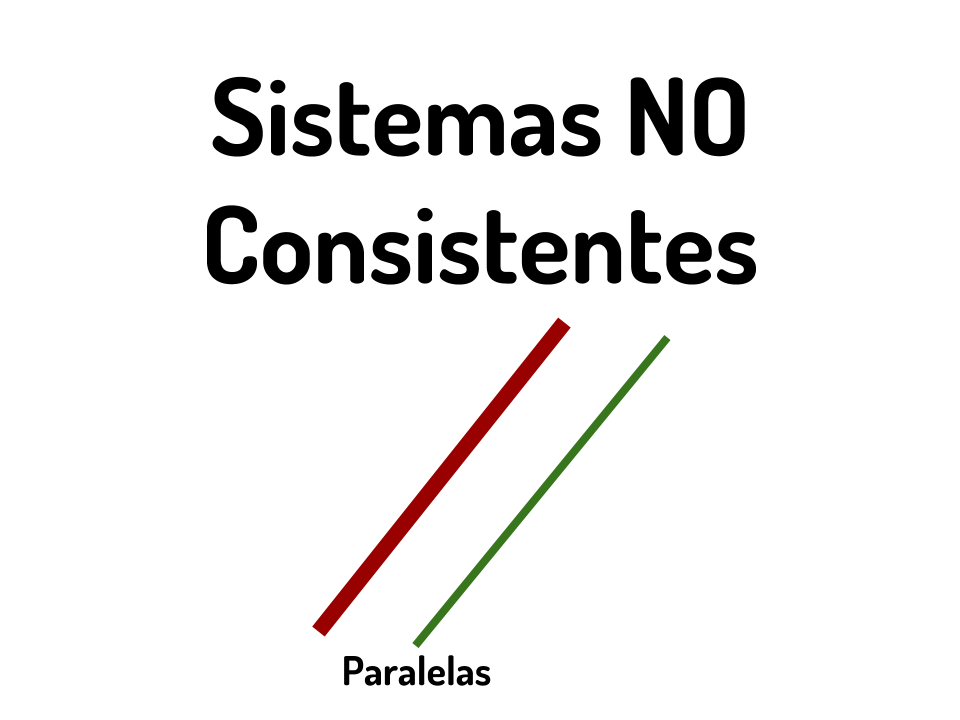
\includegraphics[width=0.60\textwidth]{SistemasNoConsistentes}
            \end{figure}




                
        % =====================================================
        % ========       SISTEMAS CONSISTENTES     ============
        % =====================================================
        \clearpage
        \section{Sistemas Consistentes}

            Podemos tener primeramente sistemas consistentes, es decir que tienen \textbf{mínimo}
            una solución.

            Es decir que las $n$ rectas (o lo que sea que sea el análogo en n-dimensiones)
            se interesectan MÍNIMO en un punto.

            Además algo muy interesante es que todo sistema homogéneo, osea que sus coeficientes
            independientes valgan cero es consistente. Donde la solución mas obvia es que
            todas las variables $x_i$ valgan CERO.

            \begin{figure}[h]
                \centering
                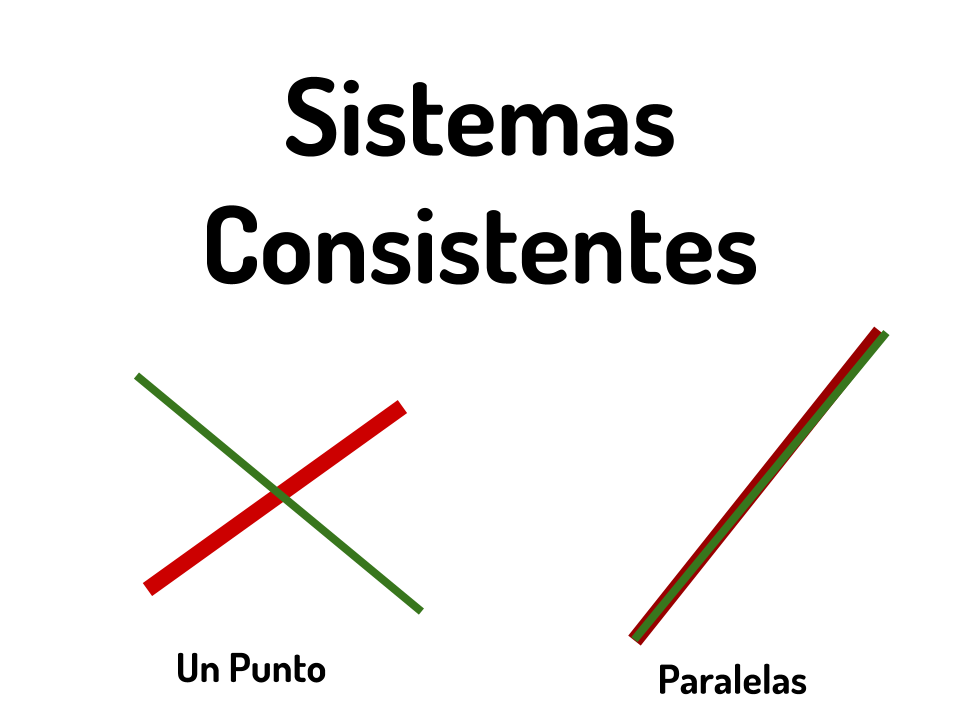
\includegraphics[width=0.60\textwidth]{SistemasConsistentes}
            \end{figure}

            
            % =====================================================
            % =======    VARIABLES PRINCIPALES Y LIBRES    ========
            % =====================================================
            \clearpage
            \subsection{Variables Principales y Libres}

                Si una matriz aumentada de un sistema de ecuaciones
                se lleva a su forma escalonada reducida por filas
                entonces decimos que:

                \begin{itemize}
                    \item \textbf{Variables Principales:}
                        Son aquellas variables que estan relacionadas
                        con un pivote
                    \item \textbf{Variables Libres:}
                        Son aquellas variables que estan relacionadas
                        con filas llenas de ceros.
                \end{itemize}


                % ======== EJEMPLO ========
                \begin{SmallIndentation}[3em]
                    \textbf{Ejemplo}:
                    Considera esta matriz escalonada reducida por filas:
                    \begin{align*}
                        \begin{bmatrix}[c c c c c c]
                            1&0&0&0&0&0                                     \\
                            0&1&0&\frac{1}{4}&\frac{-3}{4}&\frac{-3}{4}     \\
                            0&0&1&\frac{3}{4}&\frac{-1}{4}&\frac{1}{4}      \\
                            0&0&0&0&0&0
                        \end{bmatrix}
                    \end{align*}

                    Entonces podemos ver que llegamos a estas ecuaciones:
                    \begin{align*}
                        x_1 &= 0                                                \\
                        x_2 + \frac{1}{4}x_4 - \frac{3}{4}x_5 &= -\frac{3}{4}   \\
                        x_3 + \frac{3}{4}x_4 - \frac{1}{4}x_5 &= \frac{1}{4}
                    \end{align*}

                    Por lo tanto vamos a llegar a que:
                    \begin{align*}
                        x_1 &= 0                                            \\
                        x_2 &= -\frac{1}{4}r + \frac{3}{4}s - \frac{3}{4}   \\
                        x_3 &= -\frac{3}{4}r + \frac{1}{4}s + \frac{1}{4}   \\
                        x_4 &= r                                            \\
                        x_5 &= s
                    \end{align*}  

                    Es decir llegamos a que el sistema tiene una solución
                    muy bonita para cada $r, s$, \textbf{por eso las llamamos
                    variables libres}
                
                \end{SmallIndentation}
                    


            % ==================================================
            % ===   SISTEMAS CONSISTENTES  INDEPENDIENTES  =====
            % ==================================================
            \clearpage
            \subsection{Sistemas Consistentes Independientes}

                Que es lo esperado y a lo que yo llamaría normal.
                Por lo tanto si tocan en un punto entonces solo habrá una única solución.

                Esto pasa si es que no hay variables libres en el sistema.


            % ==================================================
            % ===   SISTEMAS CONSISTENTES DEPENDIENTES     =====
            % ==================================================
            \vspace{2em}
            \subsection{Sistemas Consistentes Dependientes}

                Este caso es muy especial, pues nos dice que el sistema esta
                dado por ecuaciones que son múltiplos de la otra o otra forma
                de verlo es que esta dado por vectores linealmente dependientes.

                Podemos despejar las variables principales en términos de las variables
                libres para obtener las soluciones, así que, debido a la presencia
                de variables libres el sistema tiene infinitas soluciones.























    % ===============================================================================
    % ===================    GAUSS-JORDAN Y LOS AMIGOS         ======================
    % ===============================================================================
    \clearpage
    \chapter{Gauss-Jordan y sus Amigos}



        % ==============================================
        % =====     OPERACIONES ELEMENTALES       ======
        % ==============================================
        \clearpage
        \section{Operaciones Elementales}


            % =================================================
            % =====   SWAP: INTERCAMBIAR FILAS / COL   ========
            % =================================================
            \subsection{Swap: Intercambiar Filas ó Columnas}

                La primera operación elemental es la de hacer Swap, es decir intercambiar una
                fila o columna en la matriz.
                \begin{align*}
                    &\overset{F_i \lEqual F_j}{\lLongTo}     \\
                    &\overset{C_i \lEqual C_j}{\lLongTo}
                \end{align*}

                \begin{multicols}{2}

                    % ======== DEMOSTRACION ========
                    \begin{SmallIndentation}[1em]
                        \textbf{Ejemplo de Cambio de Fila}:
                            \begin{equation*}
                                \bVector{(1)&(2)&(3)\\(4)&(5)&(6)\\7&8&9}
                                    \overset{F_1 \lEqual F_2}{\lLongTo}
                                \bVector{(4)&(5)&(6)\\(1)&(2)&(3)\\7&8&9}
                            \end{equation*}

                        \vfill
                        
                        \textbf{Ejemplo de Cambio de Columna}:
                            \begin{equation*}
                                \bVector{(1)&2&(3)\\(4)&5&(6)\\(7)&8&(9)}
                                    \overset{C_1 \lEqual F_3}{\lLongTo}
                                \bVector{(3)&2&(1)\\(6)&5&(4)\\(9)&8&(7)}
                            \end{equation*}

                    
                    \end{SmallIndentation}
                        

                \end{multicols}


                % ==================================
                % =======  MATRIZ ELEMENTAL    =====
                % ==================================
                \vspace{1em}
                \subsubsection{Matriz Elemental}

                    Podemos si queremos expresar esta operación como una \Quote{Matriz Elemental}
                    que la verdad es que no es muy útil pero la verdad es que es una forma de verlo
                    muy bonito.

                    Vamos a llamarla $SwapFilas_{a, b}$ a la matriz que es la matriz identidad pero
                    con la fila $a$ y $b$ intercambiada y $SwapColumnas_{a, b}$ a la matriz que es
                    la matriz identidad pero con la columna $a$ y $b$ intercambiada.

                    Por lo tanto para lograr el efecto de intercambiar las filas y columna haremos esto:
                    \begin{itemize}
                        \item Matriz con Cambio de Fila = $SwapFilas_{a, b} * A$
                        \item Matriz con Cambio de Columna = $A * SwapColumna_{a, b}$
                    \end{itemize}

                    Ahora, recuerda que cambiar una columna se parece mucho a intercambiar una fila y hacer
                    una transpuesta. Solo recuerda que $B^T A^T = (AB)^T$.

                    % ======== DEMOSTRACION ========
                    \begin{SmallIndentation}[1em]
                        \textbf{Ejemplo de Cambio de Fila}:
                            \begin{equation*}
                                \bVector{(1)&(2)&(3)\\(4)&(5)&(6)\\7&8&9}
                                    \overset{F_1 \lEqual F_2}{\lLongTo}
                                \bVector{(4)&(5)&(6)\\(1)&(2)&(3)\\7&8&9}
                                    \MegaSpace
                                    =
                                    \MegaSpace
                                \bVector{(0)&(1)&(0)\\(1)&(0)&(0)\\0&0&1}
                                    *
                                \bVector{1&2&3\\4&5&6\\7&8&9}
                                    =
                                \bVector{4&5&6\\1&2&3\\7&8&9}
                            \end{equation*}

                        \textbf{Ejemplo de Cambio de Columna}:
                            \begin{equation*}
                                \bVector{(1)&2&(3)\\(4)&5&(6)\\(7)&8&(9)}
                                    \overset{C_1 \lEqual F_3}{\lLongTo}
                                \bVector{(3)&2&(1)\\(6)&5&(4)\\(9)&8&(7)}
                                    \MegaSpace
                                    =
                                    \MegaSpace
                                \bVector{1&2&3\\4&5&6\\7&8&9}
                                    *
                                \bVector{(0)&0&(1)\\(0)&1&(0)\\(1)&0&(0)}
                                    =
                                \bVector{3&2&1\\6&5&4\\9&8&7}
                            \end{equation*}
                        
                    \end{SmallIndentation}



            % ==================================================
            % == PIVOT: FILAS / COL MAS MULTIPLO DE OTRA  ======
            % ==================================================
            \subsection{Pivot: Filas ó Columnas más múltiplo de otras}

                La segunda operación elemental es la de hacer Pivot, es decir a una columna sumarle
                un multiplo de otra.
                \begin{align*}
                    &\overset{F_i \lEqual F_i + nF_j}{\lLongTo}     \\
                    &\overset{C_i \lEqual C_i + nC_j}{\lLongTo}
                \end{align*}

                \begin{multicols}{2}

                    % ======== DEMOSTRACION ========
                    \begin{SmallIndentation}[1em]
                        \textbf{Ejemplo con Fila}:
                            \begin{equation*}
                                \bVector{(1)&(2)&(3)\\(4)&(5)&(6)\\7&8&9}
                                    \overset{F_1 \lEqual F_1 + 2F_2}{\lLongTo}
                                \bVector{(9)&(12)&(15)\\(4)&(5)&(6)\\7&8&9}
                            \end{equation*}

                        \vfill
                        
                        \textbf{Ejemplo con Columna}:
                            \begin{equation*}
                                \bVector{(1)&2&(3)\\(4)&5&(6)\\(7)&8&(9)}
                                    \overset{C_1 \lEqual C_1 + 1F_3}{\lLongTo}
                                \bVector{(4)&2&(3)\\(10)&5&(6)\\(16)&8&(9)}
                            \end{equation*}

                    
                    \end{SmallIndentation}
                        

                \end{multicols}


                % ==================================
                % =======  MATRIZ ELEMENTAL    =====
                % ==================================
                \vspace{1em}
                \subsubsection{Matriz Elemental}

                    Podemos si queremos expresar esta operación como una \Quote{Matriz Elemental},
                    pero esta vez, será más raro que lo normal.

                    En general $Pivot_{a, b}(k)$ es aquella matriz que nos permitirá cambiar una matriz
                    haciendo que la fila o columna $a$ sea igual a si misma más $k$ veces la fila o columna
                    $b$.

                    Vamos a llamarla $PivotFilas_{a, b}(k)$ a la matriz que es la matriz identidad
                    pero en el elemento $[PivotFilas]_{a, b}$ será igual a $k$, mientras que
                    $PivotColumnas_{a, b}(k)$ es la matriz identidad pero el elemento $[PivotColumnas]_{b, a}$
                    es igual a $k$.

                    Por lo tanto para lograr el efecto deseado haremos esto:
                    \begin{itemize}
                        \item Matriz con Pivot de Fila    = $PivotFilas_{a, b}(k) * A$
                        \item Matriz con Pivot en Columna = $A * PivotColumnas_{a, b}(k)$
                    \end{itemize}

                    % ======== DEMOSTRACION ========
                    \begin{SmallIndentation}[1em]
                        \textbf{Ejemplo de Cambio de Fila}:
                            \begin{equation*}
                                \bVector{(1)&(2)&(3)\\(4)&(5)&(6)\\7&8&9}
                                    \overset{F_1 \lEqual F_1 + 2F_2}{\lLongTo}
                                \bVector{(9)&(12)&(15)\\(4)&(5)&(6)\\7&8&9}
                                    \MegaSpace
                                    =
                                    \MegaSpace
                                \bVector{1&(2)&0\\0&1&0\\0&0&1}
                                    *
                                \bVector{1&2&3\\4&5&6\\7&8&9}
                                    =
                                \bVector{(9)&(12)&(15)\\(4)&(5)&(6)\\7&8&9}
                            \end{equation*}

                        \textbf{Ejemplo de Cambio de Columna}:
                            \begin{equation*}
                                \bVector{(1)&2&(3)\\(4)&5&(6)\\(7)&8&(9)}
                                    \overset{C_1 \lEqual C_1 + 1F_3}{\lLongTo}
                                \bVector{(4)&2&(3)\\(10)&5&(6)\\(16)&8&(9)}
                                    \MegaSpace
                                    =
                                    \MegaSpace
                                \bVector{1&2&3\\4&5&6\\7&8&9}
                                    *
                                \bVector{1&0&0\\0&1&0\\(1)&0&1}
                                    =
                                \bVector{(4)&2&(3)\\(10)&5&(6)\\(16)&8&(9)}
                            \end{equation*}
                        
                    \end{SmallIndentation}



            % ==================================================
            % =======    SCALE: ESCALAR FILAS / COL     ========
            % ==================================================
            \subsection{Scale: Escalar Filas ó Columnas}

                La tercera operación elemental es ... Ok, ok, espera, lo que pasa es que siendo
                estricto, Scale es un caso particular de Pivot donde la fila o columna de origen
                y de la destino es la misma, es decir a efectos practicos es lo mismo que escalar
                una fila o columna k veces.
                \begin{align*}
                    &\overset{F_i \lEqual nF_i}{\lLongTo}     \\
                    &\overset{C_i \lEqual nC_i}{\lLongTo}
                \end{align*}

                \begin{multicols}{2}

                    % ======== DEMOSTRACION ========
                    \begin{SmallIndentation}[1em]
                        \textbf{Ejemplo con Fila}:
                            \begin{equation*}
                                \bVector{(1)&(2)&(3)\\4&5&6\\7&8&9}
                                    \overset{F_1 \lEqual 3F_1}{\lLongTo}
                                \bVector{(3)&(6)&(9)\\4&5&6\\7&8&9}
                            \end{equation*}

                        \vfill
                        
                        \textbf{Ejemplo con Columna}:
                            \begin{equation*}
                                \bVector{1&2&(3)\\4&5&(6)\\7&8&(9)}
                                    \overset{C_3 \lEqual 2C_3}{\lLongTo}
                                \bVector{1&2&(6)\\4&5&(12)\\7&8&(18)}
                            \end{equation*}
                    
                    \end{SmallIndentation}

                \end{multicols}


                % ==================================
                % =======  MATRIZ ELEMENTAL    =====
                % ==================================
                \vspace{1em}
                \subsubsection{Matriz Elemental}

                    Podemos si queremos expresar esta operación como una \Quote{Matriz Elemental},
                    pero esta vez, será más raro que lo normal.

                    Vamos a llamarla $ScaleFilas_{i}(k)$ a la matriz que es la matriz identidad
                    pero en el elemento $[ScaleFilas]_{i, i}$ será igual a $k$, mientras que
                    $ScaleColumns_{j}(k)$ es la matriz identidad pero el elemento $[ScaleColumns]_{j, j}$
                    es igual a $k$.

                    Por lo tanto para lograr el efecto deseado haremos esto:
                    \begin{itemize}
                        \item Matriz con Scale de Fila    = $ScaleFilas_{i}(k) * A$
                        \item Matriz con Scale en Columna = $A * ScaleColumns_{j}(k)$
                    \end{itemize}

                    % ======== DEMOSTRACION ========
                    \begin{SmallIndentation}[1em]
                        \textbf{Ejemplo de Cambio de Fila}:
                            \begin{equation*}
                                \bVector{(1)&(2)&(3)\\4&5&6\\7&8&9}
                                    \overset{F_1 \lEqual 3F_1}{\lLongTo}
                                \bVector{(3)&(6)&(9)\\4&5&6\\7&8&9}
                                    \MegaSpace
                                    =
                                    \MegaSpace
                                \bVector{(3)&0&0\\0&1&0\\0&0&1}
                                    *
                                \bVector{1&2&3\\4&5&6\\7&8&9}
                                    =
                                \bVector{(3)&(6)&(9)\\4&5&6\\7&8&9}
                            \end{equation*}

                        \textbf{Ejemplo de Cambio de Columna}:
                            \begin{equation*}
                                \bVector{1&2&(3)\\4&5&(6)\\7&8&(9)}
                                    \overset{C_3 \lEqual 2C_3}{\lLongTo}
                                \bVector{1&2&(6)\\4&5&(12)\\7&8&(18)}
                                    \MegaSpace
                                    =
                                    \MegaSpace
                                \bVector{1&2&3\\4&5&6\\7&8&9}
                                    *
                                \bVector{1&0&0\\0&1&0\\0&0&(2)}
                                    =
                                \bVector{1&2&(6)\\4&5&(12)\\7&8&(18)}
                            \end{equation*}
                        
                    \end{SmallIndentation}





        % ==============================================
        % =====     ELIMINACION GAUSSIANA       ========
        % ==============================================
        \clearpage
        \section{Eliminación Gaussiana}


            % ==============================================
            % =====   MATRIZ ESCALONADA POR FILAS     ======
            % ==============================================
            \subsection{Matriz Escalonada por Filas}

                Nuestro objetivo es usando las operaciones elementales encontrar una
                forma de pasar nuestra matriz ampliada a esta forma:
                \begin{align*}
                    \textcolor{Indigo700MD}{
                        \begin{bmatrix}[lll|r]
                            1 & * & * & * \\
                            0 & 1 & * & * \\
                            0 & 0 & 1 & * 
                        \end{bmatrix}
                    }
                \end{align*}

                Ok, esto no es una definición muy matemática, estas no tienen porque
                ser matrices cuadradas, pero tienen que cumplir con las siguientes
                características:
                \begin{itemize}
                    \item 
                        Para toda fila, \textbf{si} existe un elemento distinto de cero en la fila
                        \textbf{(al que llamaremos pivote)}, entonces para todos los
                        elementos anteriores  de la fila deben ser cero y este elemento
                        \textbf{(pivote) debe ser uno, la unidad}.
                    \item
                        Los pivotes deben aparecer de forma escalonada (excepto si es que la
                        fila es nula).
                    \item
                        Si una fila no tiene pivotes entonces toda esa fila debe ser nula.
                    \item
                        Si una fila no tiene pivotes (osea que sea nula) entonces todas
                        las filas de abajo no pueden tener pivotes.
                \end{itemize}

                % =========================
                % ======== EJEMPLO ========
                % =========================
                \vspace{1em}
                \begin{SmallIndentation}[1em]
                
                    \begin{ColorText}{Red700MD}
                        \textbf{Ejemplo de Cosas que NO son}:
                        \begin{align*}
                            \bVector{2&5\\6&0}
                            \MegaSpace
                            \bVector{1&4&3\\0&1&7\\0&0&8}
                            \MegaSpace
                            \bVector{1&3&2&1\\1&-1&0&0\\0&0&1&0}
                        \end{align*}
                                
                    \end{ColorText}

                    \begin{ColorText}{Green700MD}
                        \textbf{Ejemplo de Cosas que SI son}:
                        \begin{align*}
                            \bVector{1&3&4\\0&1&7\\0&0&1}
                            \MegaSpace
                            \bVector{0&1&4\\0&0&1\\0&0&0}
                            \MegaSpace
                            \bVector{0&1&4&3\\0&0&0&1\\0&0&0&0}
                        \end{align*}
                                
                    \end{ColorText}


                \end{SmallIndentation}



            % ==============================================
            % ===========       ALGORITMO     ==============
            % ==============================================
            \clearpage
            \subsection{Algoritmo}

                \begin{enumerate}
                    \item 
                        Inicias en el primer elemento, es decir $[Matriz]_{1, 1}$
                    \item 
                        Convierte ese elemento a uno (usando la operación escalar)
                    \item
                        Usas ese uno que acabas de crear (usando la operación pivot)
                        para hacer a toda a parte de abajo de la columna sea cero
                    \item
                        Te mueves a la siguiente columna y bajas un elemento el columna
                        y repites desde el paso uno.
                \end{enumerate}




        % ==============================================
        % =====     ELIMINACION GAUSSIANA       ========
        % ==============================================
        \clearpage
        \section{Gauss-Jordan}


            % ==============================================
            % =====   MATRIZ ESCALONADA POR FILAS     ======
            % ==============================================
            \subsection{Matriz Escalonada Reducida por Filas}

                Nuestro objetivo es usando las operaciones elementales encontrar una
                forma de pasar nuestra matriz ampliada a esta forma:
                \begin{align*}
                    \textcolor{Indigo700MD}{
                        \begin{bmatrix}[lll|r]
                            1 & 0 & 0 & * \\
                            0 & 1 & 0 & * \\
                            0 & 0 & 1 & * 
                        \end{bmatrix}
                    }
                \end{align*}

                Ok, esto no es una definición muy matemática, estas no tienen porque
                ser matrices cuadradas, pero tienen que cumplir con las siguientes
                características:
                \begin{itemize}
                    \item 
                        Para toda fila, \textbf{si} existe un elemento distinto de cero en la fila
                        \textbf{(al que llamaremos pivote)}, entonces para todos los
                        elementos anteriores  de la fila deben ser cero y este elemento
                        \textbf{(pivote) debe ser uno, la unidad}.
                    \item
                        Los pivotes deben aparecer de forma escalonada (excepto si es que la
                        fila es nula).
                    \item
                        Si una fila no tiene pivotes entonces toda esa fila debe ser nula
                    \item
                        Si una fila no tiene pivotes (osea que sea nula) entonces todas
                        las filas de abajo no pueden tener pivotes.


                \end{itemize}

                % =========================
                % ======== EJEMPLO ========
                % =========================
                \vspace{1em}
                \begin{SmallIndentation}[1em]

                    \begin{ColorText}{Green700MD}
                        \textbf{Ejemplo de Cosas que SI son}:
                        \begin{align*}
                            \bVector{1&0&0\\0&1&0\\0&0&1}
                            \MegaSpace
                            \bVector{1&0&0&0\\0&0&1&0\\0&0&0&1}
                            \MegaSpace
                            \bVector{1&7&0&1&0\\0&0&1&4&0\\0&0&0&0&1\\0&0&0&0&0}
                        \end{align*}
                                
                    \end{ColorText}


                \end{SmallIndentation}



            % ==============================================
            % ===========       EJEMPLOS      ==============
            % ==============================================
            \clearpage
            \subsection{Ejemplos}
    
            \begin{SmallIndentation}[1em]
                
                % ======== EJEMPLO ========
                \textbf{Ejemplo 1}:
                    
                    Nota este sistema de ecuaciones:
                    \begin{MultiLineEquation*}{3}
                        2x_1 &-  x_2 &+ 4x_3 &= -3       \\
                         x_1 &+ 2x_2 &- 3x_3 &= 1        \\
                        5x_1 &+ 3x_2 &+  x_3 &= -2  
                    \end{MultiLineEquation*}

                    Ahora, ve esto:
                    \begin{align*}
                        \begin{bmatrix}[r r r | r]
                            2 & -1 &  4 & -3       \\
                            1 &  2 & -3 &  1       \\
                            5 &  3 &  1 & -2  
                        \end{bmatrix}
                    \end{align*}

                    Ahora, apliquemos Gauss-Jordan:
                    \begin{align*}
                        &
                        \begin{bmatrix}[r r r | r]
                            2 & -1 &  4 & -3       \\
                            1 &  2 & -3 &  1       \\
                            5 &  3 &  1 & -2  
                        \end{bmatrix}
                        &&
                        \overset{F_1 \lEqual F_2}{\lLongTo}
                        &&
                        \begin{bmatrix}[r r r | r]
                            1 &  2 & -3 &  1       \\
                            2 & -1 &  4 & -3       \\
                            5 &  3 &  1 & -2  
                        \end{bmatrix}
                        &&
                        \overset{F_2 = F_2 -2F_1}{\lLongTo}
                        &&
                        \begin{bmatrix}[r r r | r]
                            1 &  2 & -3 &  1       \\
                            0 & -5 & 10 & -5       \\
                            5 &  3 &  1 & -2  
                        \end{bmatrix}
                        \\
                        &
                        \begin{bmatrix}[r r r | r]
                            1 &  2 & -3 &  1       \\
                            0 & -5 & 10 & -5       \\
                            5 &  3 &  1 & -2  
                        \end{bmatrix}
                        &&
                        \overset{F_3 = F_3 -5F_1}{\lLongTo}
                        &&
                        \begin{bmatrix}[r r r | r]
                            1 &  2 & -3  &  1       \\
                            0 & -5 & 10  & -5       \\
                            0 & -7 & 16  & -7  
                        \end{bmatrix}
                        &&
                        \overset{F_2 = -\frac{1}{5}F_2}{\lLongTo}
                        &&
                        \begin{bmatrix}[r r r | r]
                            1 &  2 & -3  &  1       \\
                            0 & 1  & -2  & 1        \\
                            0 & -7 & 16  & -7  
                        \end{bmatrix}
                        \\
                        &
                        \begin{bmatrix}[r r r | r]
                            1 &  2 & -3  &  1       \\
                            0 & 1  & -2  & 1        \\
                            0 & -7 & 16  & -7  
                        \end{bmatrix}
                        &&
                        \overset{F_1 = F_1 -2F_2}{\lLongTo}
                        &&
                        \begin{bmatrix}[r r r | r]
                            1 & 0  & 1   & -1       \\
                            0 & 1  & -2  &  1       \\
                            0 & -7 & 16  & -7  
                        \end{bmatrix}
                        &&
                        \overset{F_1 = F_1 -2F_2}{\lLongTo}
                        &&
                        \begin{bmatrix}[r r r | r]
                            1 & 0  & 1   & -1       \\
                            0 & 1  & -2  &  1       \\
                            0 & -7 & 16  & -7  
                        \end{bmatrix}
                        \\
                        &
                        \begin{bmatrix}[r r r | r]
                            1 & 0  & 1   & -1       \\
                            0 & 1  & -2  &  1       \\
                            0 & -7 & 16  & -7  
                        \end{bmatrix}
                        &&
                        \overset{F_3 = F_3 + 7F_2}{\lLongTo}
                        &&
                        \begin{bmatrix}[r r r | r]
                            1 & 0  & 1   & -1       \\
                            0 & 1  & -2  &  1       \\
                            0 & 0  &  2  & 0  
                        \end{bmatrix}
                        &&
                        \overset{F_3 = \frac{1}{2}F_3}{\lLongTo}
                        &&
                        \begin{bmatrix}[r r r | r]
                            1 & 0  &  1  & -1       \\
                            0 & 1  & -2  &  1       \\
                            0 & 0  &  1  &  0  
                        \end{bmatrix}
                        \\
                        &
                        \begin{bmatrix}[r r r | r]
                            1 & 0  &  1  & -1       \\
                            0 & 1  & -2  &  1       \\
                            0 & 0  &  1  &  0  
                        \end{bmatrix}
                        &&
                        \overset{F_1 = F_1 - F_3}{\lLongTo}
                        &&
                        \begin{bmatrix}[r r r | r]
                            1 & 0  &  0  & -1       \\
                            0 & 1  & -2  &  1       \\
                            0 & 0  &  1  &  0  
                        \end{bmatrix}
                        &&
                        \overset{F_2 = F_2 + 2F_3}{\lLongTo}
                        &&
                        \begin{bmatrix}[r r r | r]
                            1 & 0  &  0  & -1       \\
                            0 & 1  &  0  &  1       \\
                            0 & 0  &  1  &  0  
                        \end{bmatrix}
                    \end{align*}

                    Ahora si, creo que ahora es más que obvio que:
                    \begin{align*}
                        x_1 &= -1   \\
                        x_2 &=  1   \\
                        x_3 &=  0
                    \end{align*}

            \end{SmallIndentation}
                


                    
           

        
                    
                    







        % ==============================================
        % ====        INVERSA DE UNA MATRIZ       ======
        % ==============================================
        \clearpage
        \section{Inversa de una Matriz}

            Sea $A \in M_{n \times n}(\GenericField)$ y entonces definimos a $A^{-1}$ 
            de forma informal como aquella matriz que cumple con que $A^{-1}A = AA^{-1} = I_{n}$
            nota que no para todas las matrices $M_{n \times n}(\GenericField)$ existe una matriz inversa.


           \subsubsection*{El Problema de la Notación $A^{-1}$}

           El problema con esta notación es que existen matrices no invertibles, para las cuales
           la notación $A^{-1}$ no tiene sentido.

           La notación $A^{-1}$ se puede usar solamente despúes de demostrar que $A$ es invertible.

            % ===============================
            % =========   PROPIEDADES =======
            % ===============================
            \clearpage
            \subsection{Propiedades}

                \begin{itemize}

                    \item La Matriz Inversa de $A$ ($A^{-1}$) es única.

                        % ======== DEMOSTRACION ========
                        \begin{SmallIndentation}[1em]
                            \textbf{Demostración}:

                            Lo que hay que ver que si $A,B,C \in M_n(\GenericField)$ tales que
                            $AB = BA = I_n$ y $AC = CA = I_n$. Entonces $B=C$.

                            Usando la Ley asociativa de la Multiplicación de Matrices $(A(BC)=(AB)C)$
                            tenemos que:
                            $B = B(I_n) = B(AC) = (BA)C = I_nC =  C $

                        \end{SmallIndentation}

                    \item Es necesario aunque no suficiente que todas las columnas y filas de una
                        matriz $A \in M_{n \times n}$ sea diferentes de cero para que $A$ sea invertible.

                        % ======== DEMOSTRACION ========
                        \begin{SmallIndentation}[1em]
                            \textbf{Demostración}:

                            Renglones Nulos:

                                Sea $A \in M_{n \times n}(\GenericField)$.
                                Supongamos que (por lo menos) un renglón de A es nulo, es decir:
                                $[A]_{p,*} = 0_{1,n}$ donde $0 < p \leq n$ esto es lo mismo que decir
                                que $\forall j \in \{1, \dots, n\} [A]_{p,j} = 0$.

                                Ahora supongamos que $A$ es invertible, entonces, en particular, la entrada
                                $(p,p)$ del producto $AA^{-1}$ debe coincidir con la entrada $(p,p)$ de la
                                matriz identidad $I_n$.
                                Podemos calcular esa entrada como
                                $[AA^{-1}]_{p,p} = \sum_{k=1}^{n} [A]_{p,k} [A^{-1}]_{k,p}$
                                esto debería ser $[I_n]_{p,p}=1$ pero ya vimos que $[A]_{p,k} = 0$, es decir
                                $0 = 1$. Contradicción.


                            Columnas Nulas:
                                Sea $A \in M_{n \times n}(\GenericField)$.
                                Supongamos que (por lo menos) una columna de A es nulo, es decir:
                                $[A]_{*,p} = 0_{n,1}$ donde $0 < p \leq n$ esto es lo mismo que decir
                                que $\forall j \in \{1, \dots, n\} [A]_{p,j} = 0$.

                                Ahora supongamos que $A$ es invertible, entonces, en particular, la entrada
                                $(p,p)$ del producto $A^{-1}A$ debe coincidir con la entrada $(p,p)$ de la
                                matriz identidad $I_n$.

                                Podemos calcular esa entrada como
                                $[A^{-1}A]_{p,p} = \sum_{k=1}^{n} [A^{-1}]_{p,k} [A]_{k,p}$
                                esto debería ser $[I_n]_{p,p}=1$ pero ya vimos que $[A]_{k,p} = 0$, es decir
                                $0 = 1$. Contradicción.
                            
                        \end{SmallIndentation}

                    \item Sea $A,B \in M_{m \times n}(\GenericField)$ y sean invertibles, entonces tenemos
                        que $(AB)^{-1} = B^{-1}A^{-1}$

                        % ======== DEMOSTRACION ========
                        \begin{SmallIndentation}[1em]
                            \textbf{Demostración}:

                            Si $(AB)$ es invertible entonces tenemos que probar que:
                            \begin{equation}
                            \begin{split}
                                (AB)(B^{-1}A^{-1})  &=                      \\
                                                    &= (((AB)B^{-1})A^{-1})  
                                                    &= ((A(BB^{-1}))A^{-1}) 
                                                    &= ((A(I_n))A^{-1})     
                                                    &= (AA^{-1})            \\
                                                    &= I_n 
                            \end{split}
                            \end{equation}
                            
                        \end{SmallIndentation}

                    \clearpage

                    \item Una Matriz Diagonal es invertible si y solo si los elementos de la diagonal
                        son distintos de cero.

                    \item Una Matriz Diagonal es invertible si y solo si los elementos de la diagonal
                        son distintos de cero.

                    \item Sea $A \in M_{m \times n}(\GenericField)$ y sea invertible, entonces tenemos
                        que $(A^{-1})^{-1} = A$

                    \item Sea $A \in M_{m \times n}(\GenericField)$ y sea invertible, entonces tenemos
                        que $(A^T)^{-1} = (A^{-1})^T$

                \end{itemize}
            






% //////////////////////////////////////////////////////////////////////////////////////////////////////////
% /////////////////////////////           ESPACIOS VECTORIALES        //////////////////////////////////////
% //////////////////////////////////////////////////////////////////////////////////////////////////////////
\part{Espacios Vectoriales}
\clearpage


    % ===============================================================================
    % ===================    DEFINICION Y CARACTERISTICAS         ===================
    % ===============================================================================
    \chapter{Definición y Características}

        % ==============================================
        % ========          DEFINICION            ======
        % ==============================================
        \clearpage
        \section{Definición}

            Los espacios vectoriales es la forma en que en matemáticas se abstraen conceptos clásicos como las
            fuerzas que operan en física o los polinomios con coeficientes en los reales , vamos a ver más a detalle
            esta abstracción.

            Siendo formales un Espacio Vectorial (O Espacio Lineal) es una tupla 
            $(\VectorSet, \GenericField, +, \cdot)$, solemos llamar entonces a este espacio vectorial, 
            el Espacio Vectorial de $\VectorSet$ sobre $\GenericField$ donde tenemos que:
            
            \begin{SmallIndentation}[1em]
                
                \begin{itemize}
                
                    \item
                        \textbf{Conjunto de Vectores: $\VectorSet$}

                        Es un grupo de vectores que no puede estar vacío ... y ya -.- 

                    \item
                        \textbf{Campo: $\GenericField$}

                        Es un Campo que cumple con sus propiedades normales, le solemos llamar un campo escalar.

                    \item
                        \textbf{"Suma de Vectores": $+: (\VectorSet \times  \VectorSet) \to \VectorSet$}

                        Una Función $+: (\VectorSet \times  \VectorSet) \to \VectorSet$, es decir, es una Función
                        que recibe dos elementos de $\VectorSet$ (o más específico un par ordenado de vectores) y te
                        regresa un nuevo elemento de $\VectorSet$.

                        Gracias a esto podemos decir que es cerrado en esta operación, es decir:

                        $\forall \vec{v_1}, \vec{v_2} \in \VectorSet,
                            \MiniSpace (\vec{v_1} + \vec{v_2}) \in \VectorSet$  


                    \item
                        \textbf{"Producto Escalar": $\cdot: (\GenericField \times  \VectorSet) \to \VectorSet$}

                        Una Función $\cdot: (\GenericField \times  \VectorSet) \to \VectorSet$, es decir, es una Función
                        que recibe un elementos de $\GenericField$ y un elemento de $\VectorSet$
                        (o más específico un par ordenado) y te regresa un nuevo elemento de $\VectorSet$.

                        Gracias a esto podemos decir que es cerrado en esta operación, es decir:

                        $\forall \vec{v} \in \VectorSet, \MiniSpace
                            \forall \alpha \in \GenericField, \MiniSpace
                                (\alpha \cdot \vec{v}) \in \VectorSet$  
                \end{itemize}
            
            \end{SmallIndentation}


            % ==============================================
            % ====   CONDICIONES DE ESPACIO VECTORIAL   ====
            % ==============================================
            \subsection{Condiciones de Espacio Vectorial}

                Donde esta tupla $(\VectorSet, \GenericField, +, \cdot)$ tiene que cumplir los siguientes 8
                propiedades para que se peudan considerar un espacio vectorial:

                \begin{SmallIndentation}[1em]
                    
                    \item 
                        \textbf{Ley Aditiva Asociativa:}
                        $\forall \vec{v_1}, \vec{v_2}, \vec{v_3} \in \VectorSet, \MiniSpace
                            (\vec{v_1} + \vec{v_2}) + \vec{v_3} = \vec{v_1} + (\vec{v_2} + \vec{v_3})$

                    \item 
                        \textbf{Ley Aditiva Conmutativa:}
                        $\forall \vec{v_1}, \vec{v_2} \in \VectorSet, \MiniSpace
                                \vec{v_1} + \vec{v_2} = \vec{v_2} + \vec{v_1}$

                    \item 
                        \textbf{Elemento Indentidad Aditivo:}
                        $\exists \vec{0} \in \VectorSet, \MiniSpace
                            \forall \vec{v} \in \VectorSet, \MiniSpace \vec{0} + \vec{v} = \vec{v}$

                    \item 
                        \textbf{Existen Inversos Aditivos:}
                        $\forall \vec{v} \in \VectorSet, \MiniSpace
                                \exists \vec{-v} \in \VectorSet, \MiniSpace
                                    \vec{v} + (\vec{-v}) = (\vec{-v}) + \vec{v} = \vec{0}$

                    \item 
                        \textbf{Ley Aditiva Distributiva:}
                        $\forall \alpha \in \GenericField \MiniSpace
                            \forall \vec{v_1}, \vec{v_2} \in \VectorSet \MiniSpace
                                \alpha \cdot (\vec{v_1} + \vec{v_2}) = 
                                    (\alpha \cdot \vec{v_1}) + (\alpha \cdot \vec{v_2})$

                    \item 
                        \textbf{Ley Multiplicativa Asociativa:}
                        $\forall \alpha, \beta \in \GenericField, \MiniSpace
                            \forall \vec{v} \in \VectorSet, \MiniSpace
                                \alpha \cdot (\beta \cdot \vec{v}) = (\alpha \beta) \cdot \vec{v}$

                    \item 
                        \textbf{Ley Multiplicativa Distributiva:}
                        $\forall \alpha, \beta \in \GenericField, \MiniSpace
                            \forall \vec{v} \in \VectorSet, \MiniSpace
                                (\alpha + \beta) \cdot \vec{v} = 
                                        (\alpha \cdot \vec{v}) + (\beta \cdot \vec{v})$

                    \item 
                        \textbf{Elemento Indentidad Multiplicativo:}
                        $\exists 1 \in \GenericField, \MiniSpace
                            \forall \vec{v} \in \VectorSet, \MiniSpace 1 \cdot \vec{v} = \vec{v}$

                \end{SmallIndentation}




        % =============================================
        % ============     PROPIEDADES      ===========
        % =============================================
        \clearpage
        \section{Consecuencias y Propiedades}

            Veamos algunas de las Propiedades de esto que acabamos de definir, son consecuencias de los 
            axiomas.

            \begin{itemize}
                \item El $\vec{0}$ es único.

                    % ======== DEMOSTRACION ========
                    \begin{SmallIndentation}[1em]
                        \textbf{Demostración}:

                        Si te das cuenta, nunca dije que tenia que existir solo un $\vec{0}$ pues no es
                        necesario, ya que podemos decir que si tenemos otro $\vec{0_2}$ entonces pasará que 
                        $\exists \vec{0_2} \in \VectorSet, \MiniSpace
                            \forall \vec{v} \in \VectorSet, \MiniSpace
                                \vec{0_2} + \vec{v} = \vec{v} + \vec{0_2} = \vec{v}$

                        Podemos decir entonces que $\vec{0} = \vec{0}+\vec{0_2}$ pero también sabemos como
                        funciona el $\vec{0}$, así que $\vec{0} = \vec{0}+\vec{0_2} = \vec{0_2}$.

                        Es decir, si algo cumple con querer ser nuestro cero vector, veremos que es de hecho
                        el mismo elemento.

                    \end{SmallIndentation}

                \item El inverso aditivo de $\vec{v}$ es único.

                    % ======== DEMOSTRACION ========
                    \begin{SmallIndentation}[1em]
                        \textbf{Demostración}:

                        Podemos entonces suponer que hay dos vectores $\vec{x}, \vec{y}$ que hacen el 
                        trabajo de un inverso de $\vec{v}$, es decir
                        $\vec{v} + \vec{x} = \vec{x} + \vec{v} = \vec{0}$ y que 
                        $\vec{v} + \vec{y} = \vec{y} + \vec{v} = \vec{0}$.

                        De ser así vemos entonces que podemos decir que:
                        \begin{align*}
                            \vec{x} 
                                &= \vec{x} + \vec{0}                &&\Remember{Suma de cero}   \\
                                &= \vec{x} + (\vec{v} + \vec{y})    &&\Remember{Hipotesis}      \\
                                &= (\vec{x} + \vec{v}) + \vec{y}    &&\Remember{Asociativa}     \\
                                &= \vec{0} + \vec{y}                &&\Remember{Suma de Cero}   \\
                                &= \vec{y}                          &&\Remember{Hipotesis}   
                        \end{align*}

                    \end{SmallIndentation}

                \item \textbf{Cancelación de la Suma Vectorial}:\\
                    Si $x, y, z \in \VectorSet$ tal que $x + z = y + z$, entonces $x = y$

                    % ======== DEMOSTRACION ========
                    \begin{SmallIndentation}[1em]
                        \textbf{Demostración}:

                        Esto es algo bastante natural e intuitivo, pero aun así hay que demostrarlo, 
                        veamos que $\alpha \cdot \vec{0}$ es un vector, vamos vamos a denotar su inverso
                        adivito como $- (\alpha \cdot \vec{0})$
                        \begin{align*}
                            x
                                &= x + 0            \\
                                &= x + (z + -z)     \\
                                &= (x + z) - z      \\
                                &= (y + z) - z      \\
                                &= y + (z - z)      \\
                                &= y
                        \end{align*}

                    \end{SmallIndentation}


                \clearpage


                \item $\forall \alpha \in \GenericField, \MiniSpace \alpha \cdot \vec{0} = \vec{0}$

                    % ======== DEMOSTRACION ========
                    \begin{SmallIndentation}[1em]
                        \textbf{Demostración}:

                        Esto es algo bastante natural e intuitivo, pero aun así hay que demostrarlo, 
                        veamos que $\alpha \cdot \vec{0}$ es un vector, vamos vamos a denotar su inverso
                        adivito como $- (\alpha \cdot \vec{0})$
                        \begin{align*}
                            \alpha \cdot \vec{0} 
                                &= (\alpha \cdot \vec{0}) + \vec{0}                                 \\
                                &= \alpha \cdot \vec{0} + [ (\alpha \vec{0}) - (\alpha \vec{0}) ]   \\
                                &= [\alpha \cdot \vec{0} +  (\alpha \vec{0})] - (\alpha \vec{0})    \\
                                &= [\alpha (\vec{0} + \vec{0})] - (\alpha \vec{0})                  \\
                                &= \alpha \vec{0} - (\alpha \vec{0})                                \\
                                &= \vec{0}   
                        \end{align*}

                    \end{SmallIndentation}

                \item $\forall \vec{v} \in \VectorSet, \MiniSpace 0 \cdot \vec{v} = \vec{0}$

            \end{itemize}




    % ===============================================================================
    % ===================    SUB ESPACIOS VECTORIALES             ===================
    % ===============================================================================
    \chapter{Subespacios Vectoriales}

        % ==============================================
        % ========          DEFINICION            ======
        % ==============================================
        \clearpage
        \section{Definición}

            Suele ser muy interasante ver si es que los subconjuntos de cierta estructura
            algebraica tienen las mismas características, por lo tanto veamos si es que
            podemos encontrar un subconjunto de un espacio vectorial.

            Un Subespacio Vectorial es un Espacio Vectorial.

            La única razón por la que le decimos Subespacio es porque esta contenido dentro de
            otro Espacio Vectorial.

            % ==============================================
            % ========      DEFINICION FORMAL    ===========
            % ==============================================

            \subsubsection{Definición Formal}
                Sea $\SubVectorSet$ y $\VectorSet$ dos Espacios Vectoriales donde con identidas
                operaciones $+, \cdot$ sobre un mismo campo $\GenericField$ entonces decimos
                que $\SubVectorSet$ es un Subespacio Vectorial de $\VectorSet$ si y solo si:

                \begin{itemize}
                    \item $\SubVectorSet \subset \VectorSet$
                    \item $\SubVectorSet$ es un Espacio Vectorial por si mismo
                \end{itemize}


        % ==============================================
        % ====     DEMOSTRAR QUE ES UN SUBESPACIO   ====
        % ==============================================
        \vspace{1em}
        \section{Demostrar que $\SubVectorSet$ es un Subespacio de $\VectorSet$}

            Afortunadamente no tenemos que demostrar todas las 8 propiedades de un espacio
            vectorial, porque después de todo es un subconjunto de $\VectorSet$. Por lo tanto
            solo basta probar algunas menos.

            Podemos además decir que $\SubVectorSet$ es un Subespacio de $\VectorSet$
            si y solo si:

            $\SubVectorSet$ contiene al vector cero del Espacio $\VectorSet$ y es cerrado
            con respecto a las operaciones lineales del Espacio $\VectorSet$, (osea con
            expresiones matemáticas:)

            \begin{itemize}
                \item $\vec{0} \in \SubVectorSet$
                
                \item $\forall \vec{v_1}, \vec{v_2} \in \SubVectorSet, \MiniSpace
                            \vec{v_1} + \vec{v_2} \in \SubVectorSet$

                \item $\forall \vec{v} \in \SubVectorSet, \MiniSpace
                            \forall \alpha \in \GenericField, \MiniSpace
                                \alpha \vec{v} \in \SubVectorSet$
            \end{itemize}

            A veces hay gente que le gusta poner una 4 condición, la de que
            $\forall \vec{v} \in \SubVectorSet, \MiniSpace -\vec{v} \in \SubVectorSet$, pero la verdad
            es que podemos probar que esta cuarta condición se puede probar usando las 3 anteriores.



        % ==============================================
        % ==========     PROPIEDADES    ================
        % ==============================================
        \vspace{1em}
        \section{Propiedades de los Subespacios}

            \begin{itemize}
                
                \item 
                    $\Set{ \vec{0} }$ es un Subespacio Vectorial para cualquier $\VectorSet$

                \item
                    Cualquier intersección de Subespacios Vectoriales de $\VectorSet$ es también un
                    Subespacio Vectorial de $\VectorSet$

                    % ======== DEMOSTRACION ========
                    \begin{SmallIndentation}[1em]
                        \textbf{Demostración}:
                        
                        Sea $\SubVectorSet$ la intersección de 2 subespacios vectoriales $A$ y $B$ cualquiera
                        entonces:

                        \begin{itemize}
                            \item Es obvio que $\SubVectorSet$ contiene al $\vec{0}$, porque estaba tanto
                                es $A$ como $B$ por ser subespacios.

                            \item Sea $\vec{v_1}, \vec{v_2} \in \SubVectorSet$ entonces estos 2 elementos
                                existen en cada subespacio y como son subespacios entonces 
                                $\vec{v_1} + \vec{v_2} \in \SubVectorSet$

                            \item Sea $\vec{v} \in \SubVectorSet$ entonces $\vec{v}$ existe en ambos subespacios
                                y como son subespacio entonces 
                                $\forall \alpha \in \GenericField, \alpha \vec{v} \in \SubVectorSet$

                        \end{itemize}

                        Por lo tanto, es un subespacio vectorial.
                    
                    \end{SmallIndentation}

                \item
                    Cualquier unión de Subespacios Vectoriales de $\VectorSet$ es también un
                    Subespacio Vectorial de $\VectorSet$ si y solo si uno de los subespacios
                    es un subconjunto de otro
                        

            \end{itemize}



        % ==============================================
        % ======     SUMA DE SUBESPACIOS      ==========
        % ==============================================
        \clearpage
        \section{Suma de Subespacios Vectoriales}

            Si $S_1$ y $S_2$ son subespacios vectoriales (que no son vacios) de un Espacio Vectorial
            $\VectorSet$, entonces definimos a $S_1 + S_2$ de la siguiente manera:

            \begin{align}
                S_1 + S_2 := \Set{
                    \vec x 
                        \Such \vec x = \vec{a} + \vec{b} 
                        \Space \text{donde} \Space
                        \vec{a} \in S_1 \text{ y }
                        \vec{b} \in S_2
                    }
            \end{align}


            % ==============================================
            % ==========     PROPIEDADES    ================
            % ==============================================
            \vspace{1em}
            \subsection{Propiedades}

                \begin{itemize}
                    
                    \item 
                        Si $\SubVectorSet_1$ y $\SubVectorSet_2$ son subespacios de un espacio vectorial de
                        $\VectorSet$ entonces $\SubVectorSet_1 + \SubVectorSet_2$ es un Subespacio Vectorial

                            % ======== DEMOSTRACION ========
                            \begin{SmallIndentation}[1em]
                                \textbf{Demostración}:
                                
                                \begin{itemize}
                                    \item Por un lado como $\SubVectorSet_1$ y $\SubVectorSet_2$ son subespacios
                                        entonces $\vec{0} + \vec{0}$ esta en la suma, por lo tanto el $\vec{0}$
                                        esta.

                                    \item Sea $a, b \in \SubVectorSet_1 + \SubVectorSet_2$, además podemos
                                        proponer elementos tales que $x_1, y_1 \in \SubVectorSet_1$ y 
                                        $x_2, y_2 \in \SubVectorSet_2$ tales que $a=x_1+x_2$ y $b=y_1+y_2$
                                        entonces:
                                        \begin{align*}
                                            a + b
                                                &= (x_1 + x_2) + (y_1 + y_2)    \\ 
                                                &= (x_1 + y_1) + (x_2 + y_2)    \\ 
                                                &= (x_1 + y_1) + (x_2 + y_2)    \\ 
                                        \end{align*}

                                        Es decir $a+b$ es un elemento de $\SubVectorSet_1 + \SubVectorSet_2$

                                    \item $ax = a(x_1 + x_2) = ax_1 + a_x2$
                                        es un elemento de $\SubVectorSet_1 + \SubVectorSet_2$

                                \end{itemize}
                            
                            \end{SmallIndentation}

                \end{itemize}




            % ==============================================
            % ======     SUMA DE SUBESPACIOS      ==========
            % ==============================================
            \clearpage
            \subsection{Suma Directa de Subespacios Vectoriales}

                Se dice que $\VectorSet$ es la suma directa de $\SubVectorSet_1$ y $\SubVectorSet_2$
                expresada como $\VectorSet = \SubVectorSet_1 \oplus \SubVectorSet_2$ si y solo si:

                \begin{itemize}
                    \item $\SubVectorSet_1, \SubVectorSet_2$ son subespacios vectoriales de $\VectorSet$
                    \item $\SubVectorSet_1 \cap \SubVectorSet_2 = \Set{\vec{0}}$
                    \item $\VectorSet = \SubVectorSet_1 + \SubVectorSet_2$
                \end{itemize}


            % ==============================================
            % ==========     PROPIEDADES    ================
            % ==============================================
            \vspace{1em}
            \subsubsection{Propiedades}

                \begin{itemize}
                    
                    \item 
                        $\VectorSet$ es la suma directa de $\SubVectorSet_1$ y $\SubVectorSet_2$ si y solo si
                        cada elemento $x$ de $\VectorSet$ puede ser escrito de una sola manera como 
                        $x = a + b$ donde $a \in \SubVectorSet_1$ y $b \in \SubVectorSet_2$

                \end{itemize}

\end{document}